\documentclass[ms,electronic,twosidetoc,letterpaper,chaptercenter,parttop,lol,lof,lot]{byumsphd}
% Author: Chris Monson
%
% This document is in the public domain
%
% Options for this class include the following (* indicates default):
%
%   phd (*) -- produce a dissertation
%   ms -- produce a thesis
%
%   electronic -- default official university option, overrides the following:
%                 - equalmargins
%
%   hardcopy -- overrides the following:
%                 - no equalmargins
%                 - twoside
%
%   letterpaper -- ignored, but helpful for the Makefile that I use
%
%   10pt -- 10 point font size
%   11pt -- 11 point font size
%   12pt (*) -- 12 point font size
%
%   lof -- produce a list of figures in the preamble (off)
%   lot -- produce a list of tables in the preamble (off)
%   lol -- produce a list of listings in the preamble (off)
%
%   layout -- show layout lines on the pages, helps with overfull boxes (off)
%   grid -- show a half-inch grid on every page, helps with printing (off)
%   separator -- print an extra instruction page between preamble and body (off)
%
%   twoside (*) -- two-sided output (margins alternate for odd and even pages,
%     blank pages inserted to ensure that chapters begin on the right side of a
%     bound copy, etc.)
%   oneside -- one-sided output (margins are the same on all pages)
%   equalmargins -- make all margins equal - ugly for binding, but compliant
%
%   twosidetoc - start two-sided margins at the TOC instead of the body.  This
%     is sometimes (oddly) required, but be aware that it will make the page
%     numbering seem screwy, e.g., the first four full sheets of paper will
%     have number i-iv (not shown, though), and the next sheets will each have
%     two numbers, one for each side.  I suspect that most people don't look at
%     the roman numerals anyway, but it is a weird requirement.
%
%   openright (*) -- force new chapters to start on an odd page
%   openany -- don't use this, it's ugly
%
%   prettyheadings -- make the section/chapter headings look nice
%   compliantheadings (*) -- make them look ugly, but compliant with standards
%
%   chaptercenter -- center the chapter headings horizontally
%   chapterleft (*) -- place chapter headings on the left
%
%   partmiddle -- Part headers are centered vertically, no other text on page
%   parttop (*) -- Part headers at top of page, other text expected
%
%   duplexprinter -- Ensures that the two-sided portion starts on the right
%     side when printing.  This is not for use in submission, since the best
%     thing to do there is to print everything out one-sided, then take it down
%     to the copy store to have them do the rest.  It does help to save trees
%     when you are printing out copies just to look at them and fiddle with
%     things.
%
%
% EXAMPLES:
%
% The rest is up to you.  To fiddle with margins, use the \settextwidth and
% \setbindingoffset macros, described below.  I suggest that you
% \settextwidth{6.0in} for better-looking output (otherwise you'll get 3/4-inch
% margins after binding, which is sort of weird).  This will depend on the
% opinions of the various dean/coordinator folks, though, so be sure to ask
% them before embarking on a major formatting task.

% The following command fixes my particular printer, which starts 0.03 inches
% too low, shifting the whole page down by that amount.  This shifts the
% document content up so that it comes out right when printed.
%
% Discovering this sort of behavior is best done by specifying the ``grid''
% option in the class parameters above.  It prints a 1/2 inch grid on every
% page.  You can then use a ruler to determine exactly what the printer is
% doing.
%
% Uncomment to shift content up (accounting for printer problems)
%\setlength{\voffset}{-.03in}

% Here we set things up for invisible hyperlinks in the document.  This makes
% the electronic version clickable without changing the way that the document
% prints.  It's useful, but optional.
%
% NOTE: "driverfallback=ps2pdf" chooses ps2pdf in the case of LaTeX and pdftex
% in the case of pdflatex. If you use my LaTeX makefile (at
% http://latex-makefile.googlecode.com/) then pdftex is the default There are
% many other benefits to using the makefile, too.  This option is not always
% available, so use with care.
\usepackage[
    bookmarks=true,
    bookmarksnumbered=true,
    breaklinks=false,
    raiselinks=true,
    pdfborder={0 0 0},
    colorlinks=false,
    plainpages=false,
    ]{hyperref}

\usepackage{graphicx}
\usepackage{caption}
\usepackage{subcaption}
\usepackage{float}
\usepackage{scrextend}
\usepackage{url}
%\usepackage{courier}
\usepackage{titlesec}
\usepackage[]{algorithm2e}
\usepackage{amsmath}
\usepackage{titlesec}

\setcounter{secnumdepth}{4}

% To fiddle with the margin settings use the below.  DO NOT change stuff
% directly (like setting \textwidth) - it will break subtle things and you'll
% be tearing your hair out.
%
% For example, if you want 1.5in equal margins, or 2in and 1in margins when
% printing, add the following below:
%
%\setbindingoffset{1.0in}
%\settextwidth{5.5in}
%
% When equalmargins is specified in the class options, the margins will be
% equal at 1.5in each: (8.5 - 5.5) / 2.  When equalmargins is not specified,
% the inner margin will be 2.0 and the outer margin will be 1.0: inner = (8.5 -
% 5.5 - 1.0) / 2 + 1.0 (the 1.0 is the binding offset).
%
% The idea is this: you determine how much space the text is going to take up,
% whether for an electronic document (equalmargins) or not.  You don't want the
% layout shifting around between printed and electronic documents.
%
% So, you specify the text width.  Then, if there is a binding offset (when
% binding your thesis, the binding takes up space - usually 0.5 inches), that
% reduces the visual space on the final printed copy.  So, the *effective*
% margins are calculated by reducing the page size by the binding offset, then
% computing the remaining space and dividing by two.  Adding back in the
% binding offset gives the inner margin.  The outer margin is just what's left.
%
% All of this is done using the geometry package, which should be manipulated
% directly at your peril.  It's best just to use the above macros to manipulate
% your margins.
%
% That said, using the geometry macro to set top and bottom margins, or
% anything else vertical, is perfectly safe and encouraged, e.g.,
%
%\geometry{top=2.0in,bottom=2.0in}
%
% Just don't fiddle with horizontal margins this way.  You have been warned.

% This makes hyperlinks point to the tops of figures, not their captions
\usepackage[all]{hypcap}

% These packages allow the bibliography to be sorted alphabetically and allow references to more than one paper to be sorted and compressed (i.e. instead of [5,2,4,6] you get [2,4-6])
\usepackage[numbers,sort&compress]{natbib}
\usepackage{hypernat}

% Because I use these things in more than one place, I created new commands for
% them.  I did not use \providecommand because I absolutely want LaTeX to error
% out if these already exist.
\newcommand{\Title}{Subword Spotting and its Applications}
\newcommand{\Author}{Brian L.~Davis}
\newcommand{\GraduationMonth}{December}
\newcommand{\GraduationYear}{2017}

% Set up the internal PDF information so that it becomes part of the document
% metadata.  The pdfinfo command will display this.
\hypersetup{%
    pdftitle=\Title,%
    pdfauthor=\Author,%
    pdfsubject={MS Thesis, BYU CS Department: %
                Degree Granted \GraduationMonth~\GraduationYear, Document Created \today},%
    pdfkeywords={subword, spotting, CAT, semi-automated, handwriting},%
}

% Rewrite the itemize, description, and enumerate environments to have more
% reasonable spacing:
\newcommand{\ItemSep}{\itemsep 0pt}
\let\oldenum=\enumerate
\renewcommand{\enumerate}{\oldenum \ItemSep}
\let\olditem=\itemize
\renewcommand{\itemize}{\olditem \ItemSep}
\let\olddesc=\description
\renewcommand{\description}{\olddesc \ItemSep}

% Important settings for the byumsphd class.
\title{\Title}
\author{\Author}

\committeechair{William Barrett}
\committeemembera{Thomas Sederberg}
\committeememberb{Daniel Zappala}

\monthgraduated{\GraduationMonth}
\yeargraduated{\GraduationYear}
\yearcopyrighted{\GraduationYear}

\documentabstract{%
This is where the abstract goes.

Note that there is a blank line between paragraphs, here. 
X==================
=====================
==================
}

\documentkeywords{%
	subword, spotting, CAT, semi-automated, handwriting
}

\acknowledgments{%
    I would like to thank my wife Sarah for her patience with and support of my endeavors.
}

\department{Computer~Science}
\graduatecoordinator{Christophe Giraud-Carrier}
\collegedean{Thomas~W.~Sederberg}
\collegedeantitle{Associate~Dean}

% Customize the name of the Table of Contents section.
\renewcommand\contentsname{Table of Contents}

% Remove all widows an orphans.  This is not normally recommended, but in a
% paper dissertation there is no reasonable way around it; you can't exactly
% rewrite already-published content to fix the problem.
\clubpenalty 10000
\widowpenalty 10000

% Allow pages to have extra blank space at the bottom in order to accommodate
% removal of widows and orphans.
\raggedbottom

% Produce nicely formatted paragraphs. There is nothing additional to do.  In
% case you get some problems, surround your text with
% \begin{sloppy} ... \end{sloppy}. If that does not work, try
% \microtypesetup{protrusion=false} ... \microtypesetup{protrusion=true}
\usepackage{microtype}

\begin{document}

% Produce the preamble
\microtypesetup{protrusion=false}
\maketitle
\microtypesetup{protrusion=true}

%%%%%%%%%%%%%%%%%%%%%%%%%%%%%%%%%%%%%%%%%%%%%%%%%%%%%%%%%%%%%%%%%%%%%%%%%%%%%%
\chapter{Introduction}

Most data recorded by humans in the past, and much even today, is in handwritten documents. 
It is highly desirable for many areas of research for this information to be easily accessible, either being searchable through automatic means or having the data digitized in some form that is easily manipulated by computers.

The digitization of these documents is a large task. Obviously not all recorded data is important, but even within a specific domain, the number of relevant handwritten documents can be far too large to be manually transcribed to digital text (that is, a human reads the document and then types the contents into a computer). Within the domain of family history research there are billions of handwritten documents which have been photographed as digital images and more are being captured every day.
%which would be easily searchable if they were transcribed to digital text. Digitized records also can facilitate automated information extraction (e.g.~relationships between people for genealogical purposes). A mighty effort has been underway to capture many of these documents as digital images, but 
The transcription of these lags far behind, and the gap is growing. It is an expensive task to have the contents of these documents manually typed by people.

A solution to the problem of transcribing documents that has been worked on for several decades is automated handwriting recognition. The basic formulation is that given an image of handwriting (either a character, word, line, paragraph or page), automatically produce the text of its handwritten content. The state-of-the art is primarily focused on the transcription of text lines and paragraphs through artificial neural networks, particularly recursive neural networks (RNN) \cite{icfhrComp2016, wigington2017, icdarComp2017}. These methods work relatively well, particularly in single author scenarios. However, they do require large training sets and would require human correction in some difficult applications where human-level accuracy is required.

Computer assisted transcription (CAT), or semi-automated transcription, is an approach to transcription which begins with the understanding that human input will be needed to achieve the desired accuracy and aims to merge computed and human effort in an effective manner. 
These methods have generated less interest recently due to the large gains deep convolutional neural networks have given automatic transcription.

However, transcription is not always needed; if search is the only utility desired an alternative solution is word spotting \cite{manmatha1996}. In word spotting, the goal is to make a collection of document images searchable without transcription. The search results are based on visual features the system extracts. The result of word spotting is the location, and potentially bounding box, of all instances of the query (see Figure \ref{fig:explain_spotting}). 

\begin{figure}[t]
    \begin{subfigure}{0.46\textwidth}
    		\centering
    		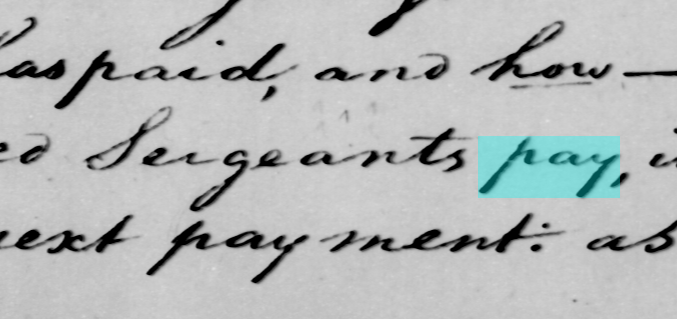
\includegraphics[width=\textwidth]{spotting_explination_pay}
    		%\caption{A small window shows the user matching words later in the column. The user can get rid of bad matches by either clicking on them or adjusting a  threshold.}
    	\end{subfigure}
    	~
    	\begin{subfigure}{0.46\textwidth}
    		\centering
    		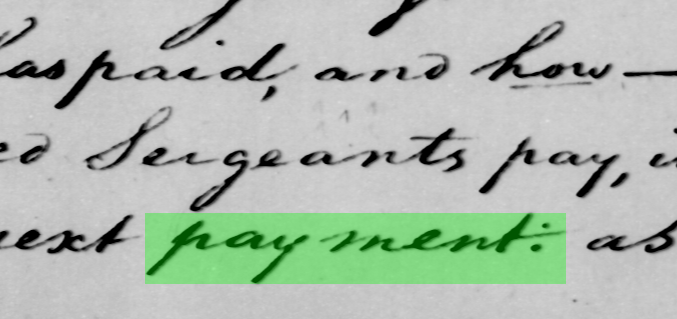
\includegraphics[width=\textwidth]{spotting_explination_payment}
    		%\caption{The matched words are given the same label when entered.}
    	\end{subfigure}
    	\caption{Examples of word spotting for `pay' and `payment'.}
    	\label{fig:explain_spotting}
\end{figure}

\begin{figure}[t]
    \begin{subfigure}{0.46\textwidth}
    		\centering
    		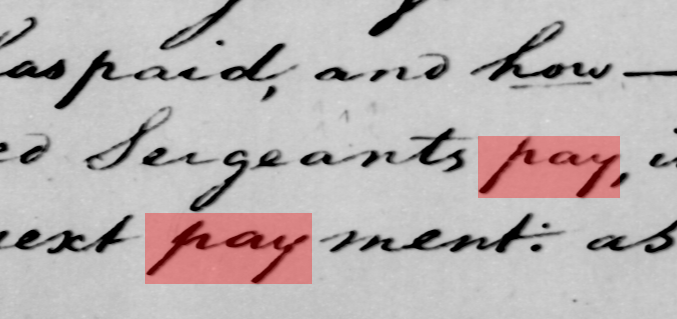
\includegraphics[width=\textwidth]{spotting_explination_sub_pay}
    		%\caption{A small window shows the user matching words later in the column. The user can get rid of bad matches by either clicking on them or adjusting a  threshold.}
    	\end{subfigure}
    	~
    	\begin{subfigure}{0.46\textwidth}
    		\centering
    		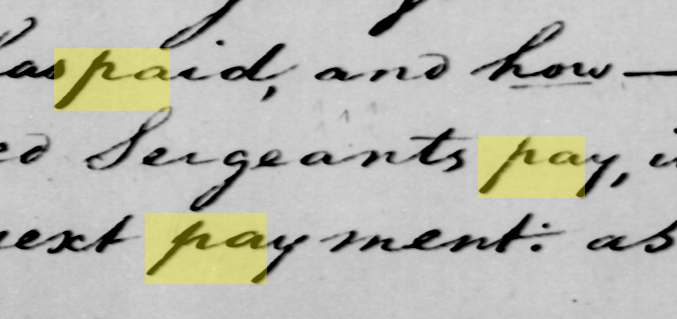
\includegraphics[width=\textwidth]{spotting_explination_sub_pa}
    		%\caption{The matched words are given the same label when entered.}
    	\end{subfigure}
    	\caption{Examples of subword spotting for the character trigram `pay' (left, red) and bigram `pa' (right, yellow).}
    	\label{fig:explain_sub_spotting}
\end{figure}

In this work, subword spotting is explored. Where word spotting finds words matching a query, subword spotting relaxes this to finding any instances of the query, even within a word. As seen in Figure \ref{fig:explain_sub_spotting} (left, red), an additional instance of ``pay'' is found compared to Figure \ref{fig:explain_spotting}.
And in Figure \ref{fig:explain_sub_spotting} (right, yellow), an additional instance of ``pa'' is found, which turns out to be a different form of the word``pay''.
%Of interest in subword spotting are atomic units of words which occur...



%The scope of this thesis is to use subword spotting (looking for groups of characters within words) as the back-bone of a CAT system. This aims to break the transcription task, from a user perspective, to micro-tasks that can be completed easily with a smartphone. For any CAT system to be considered successful, it must be faster than manual transcription while achieving comparable accuracy.

\section{Why Subword Spotting?}

The original motivation for exploring subword spotting came from the observation that techniques for handwriting recognition have tried many different primitives, or fundamental units, for recognition. One can look at pixels at the lowest level, and then move onto graphemes or substrokes \cite{liang2012}, strokes, characters, subwords (or character n-grams), words and sentences. With current neural networks, the primitives are learned within the stacked convolutional layers, and the network then recognizes characters based on these. Previous CAT systems such as \cite{Clawson2014} and \cite{Zagoris2015} use whole words as units for recognition. 

%Subwords provide an interesting middle ground between these units. Characters can be very similar to one another (in cursive ``i'' missing it's dot frequently looks like an ``e'') making discriminating between them very difficult. Words, on the other hand, can occur very infrequently, such as names which occur once in an entire corpus. Subwords occur frequently while providing more context than single characters and thus may be a primitive well suited to handwritting.


An individual primitive has two desirable properties: distinctiveness and frequency. Without distinctiveness it will be very difficult to discriminate between different primitive instances. Frequency is valuable as it allows us to get more out of the effort required to discriminate, or potentially the effort required to learn how to discriminate.

Subwords provide an interesting middle ground between individual characters and complete words. %, each of these having flaws improved upon by subwords.
Individual characters can be very similar to one another (i.e.~not distinctive). For example, in cursive an ``i'' missing it's dot frequently looks like an ``e'', as seen in Figure \ref{fig:ei}, making discriminating between characters in isolation very difficult. On the other hand, words are generally much more distinctive than characters. However, while individual characters occur many times throughout a corpus, a given word may appear less frequently. In the extreme, words such as names, may occur only once. However, subwords, such as ``th'', ``ed'', ``ion'', ``ing'', etc., occur very frequently (in English) as they are used in many words. And while being more frequent than words, subwords also provide more distinctiveness and discernibility than individual characters.

\begin{figure}
    \centering
    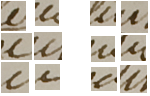
\includegraphics[width=0.45\textwidth]{ei}
    \caption{Cropped examples of the characters ``e'' and ``i'' (excluding dots), on the left and right respectively, from a single author. Without context the characters are practically indistinguishable.}
    \label{fig:ei}
\end{figure}

Important use cases for subword spotting include searches (1) where a root is desired to be searched, such as querying ``pay'' wanting to find instances of ``payment'', ``payments'', ``prepay'', etc., (2) where only part of the desired word, such as a name, is known, such as ``Chr.'', (3) where there are character(s) which a human transcriber cannot initially recognize, but if instances elsewhere in the document in familiar words could be found in context, would become discernible to the transcriber.

An additional appeal of subword spotting lies in computer assisted transcription (CAT). In character-level recognition schemes, a lexicon is frequently used to correct erroneous character predictions if other characters in the word are transcribed correctly. Similarly a lexicon can also be used to fill in untranscribed characters, assuming significant other characters are transcribed. This is useful in a transcription by iteratively spotting subwords. While the spotting results may not cover every character, they can cover a sufficient number of characters for each particular word.

In Figure \ref{fig:subtransexample} we see an example of the word ``payment'', where ``pa'' and ``men'' have been spotted; this covers 71\% of the characters in the word. However, if we estimate that there are 1-2 characters between ``pa'' and ``men'' and estimate 1-2 characters after ``men'' the regular expression \texttt{pa..?men..?} matchs only ``pavement'', ``pavements'', ``payment'', and ``payments'' in our large lexicon (described in Chapter \ref{datasets}). This is a particularly potent tool with longer words, which typically may require more effort to automatically transcribe, but tend to be more distinctive from a lexical perspective.

\begin{figure}
    \centering
    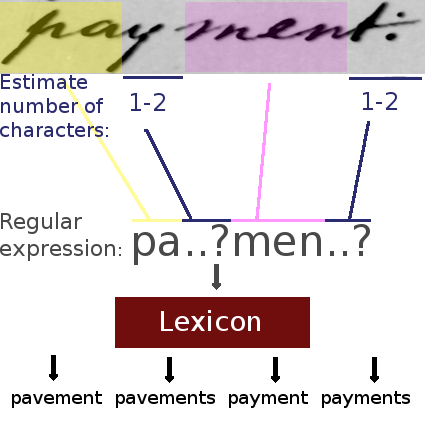
\includegraphics[width=0.55\textwidth]{spotting_completion_payment}
    \caption{An example of a word having ``pa'' and ``men'' spotted in it. A regular expression representing this, \texttt{pa..?men..?}, yields only a few matches from our lexicon, including the correct one: ``pavement'', ``pavements'', ``\textbf{payment}'', and ``payments''.}
    \label{fig:subtransexample}
\end{figure}

%While these previous motivations are based on transcription, subword spotting has a the potential to be a more flexible search tool than word spotting is. In this work we show this in the application of searching for words with specific suffixes.

\section{Main Contributions}

The primary scope of this work is to provide an exploration of the performance of subword spotting, extending state-of-the-art word spotting methods.
We show that reasonable levels of mean average precision (MAP) can be achieved for character tri-, bi-, and unigram spotting. We demonstrate the variability in performance between different character n-grams (referred to as simply n-grams hereafter).

Additionally, we demonstrate several applications of subword spotting: user directed searching to aid in human transcription, suffix searching/spotting, and CAT using word completion from aggregated subword spottings.

%%%%%%%%%%%%%%%%%%%%%%%%%%%%%%%%%%%%%%%%%%%%%%%%%%%%%%%%%%%%%%%%%%%%%%%%%%%%%%
\chapter{Related Work}\label{relatedwork}

\section{Word Spotting}\label{relatedwork_wordspotting}


Word spotting was first proposed as an alternative to transcribing a corpus. Rather than transcribing the document image so standard text searches can be run, the document is searched using the images themselves, either with a keyword string or a keyword image (exemplar image). In the past, techniques were distinguished by which search pattern they used. There are two primary approaches to featurizing the images when word spotting is performed: holistic features, that capture information about a whole image (word), and local or sequential features \cite{Rodrıguez2008}. Holistic features have one description for an entire word image (such as a bag-of-visual-words \cite{Shekhar2012}), whereas local features have a descriptor for a small portion, or window, of a word image. 
%Because local features provide much more detail and are more flexible than holistic features, they have been the most actively pursued in research.

Most early work with local features share the common theme of taking features from vertical slice windows (usually only one or a handful of pixels wide); Figure \ref{fig:vertslice} shows an example of this process. They compare these to a the features extracted from an exemplar using either dynamic time warping or hidden Markov models (HMMs), relying on a prior line segmentation. The variation between the methods largely lies in the features used. Some use small square windows to allow segmentation-free word spotting using a sliding window \cite{Rothacker2013}.

\begin{figure}[t]
    \centering
    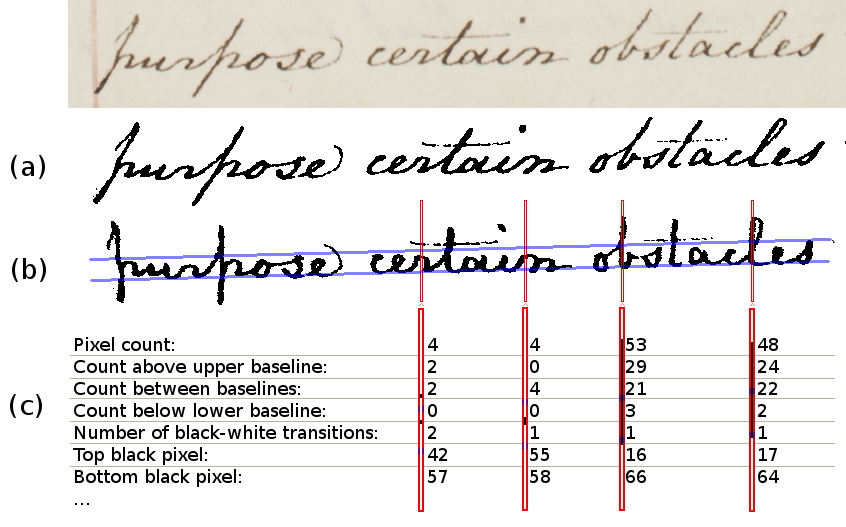
\includegraphics[width=.9\textwidth]{vertwind}
    \caption{Example of how vertical slice window features are extracted. Typically most features are extracted on a binarized image. Deskewing plays an important role as the vertical slices are very sensitive to skew. Many features extracted are pixel counts; in this example we show count features dependent on baselines (blue).}
    \label{fig:vertslice}
\end{figure}

Rodr{\i}guez et al.~\cite{Rodrıguez2008} proposed a simple histogram gradient feature that demonstrated improved performance when compared with (1) the popular profile and transition-based features of Rath and Manmantha \cite{Rath2003}, (2) the gradient and transition-focused features of Marti and Bunke \cite{Marti2001} and (3) the simple histogram features of Bunke et al.~\cite{Bunke2004}. They also showed that a HMM worked better than dynamic time warping, for their features. Their method was not an exemplar-based approach.

Aldavert et al.~\cite{Aldavert2015} and Almazan et al.~\cite{Almazan2014} have presented superior word spotting methods that rely on heuristic descriptions. Aldavert et al.~used the well known bag-of-visual-words method, including recent improvements from the computer vision community. This is a very simple, yet effective, exemplar spotting approach. Aldavert et al.~use Fischer vectors, which are similar to bag-of-visual-words, with spatial pyramids in addition to a special pyramidal histogram of characters (PHOC).
% which are described in more detail in Chapter \ref{subwordspotting}. 
PHOC vectors are a fixed length vector which describe a word; it encodes which characters are present and roughly their location. If your alphabet is length $N$, the first $N$ values of the vector indicate if each character is present in the word (Is `a' in the word? Is `b' in the word?). The next $N$ values indicate if each character is present in the first half of the word, the $N$ values after that indicating presence in the second half of the word. This is carried out to three levels, and a set of character bigrams are also used on the first two levels. See Figure \ref{fig:phoc} for clarification.
The PHOC vector and pyramidal bag-of-visual-words are used to find a new space in training in which both strings and word images can be embedded. This allows it to perform both string and exemplar queries as well as hybrid queries which yield excellent results.

\begin{figure}[t]
    \centering
    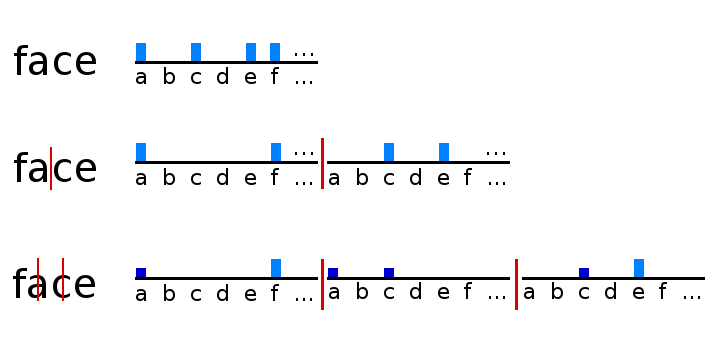
\includegraphics[width=.65\textwidth]{phoc}
    \caption{Example of a three level PHOC vector for the word ``face''. The final vector is all levels appended together. Note that partial values are given when characters are split over bins.}
    \label{fig:phoc}
\end{figure}

%PHOCNet
Sudholt and Fink \cite{sudholt2016,sudholt2017} expanded on \cite{Almazan2014} by training a deep convolutional neural network to produce the PHOC vector from a word image. This, and following improvements \cite{krishnan2016, retsinasTrans2017}, have yielded the state-of-the-art for segmentation based spotting. We base our spotting method on \cite{sudholt2017}.

There are also techniques for segmentation-free word spotting, where they don't require segmented word images but can use full page images \cite{wilkinson2017}. While we used word image segmentations in our work to narrow its scope, we note that it could be applied, with some adjustments, in a segmentation-free setting.

We are interested in spotting character n-grams (uni-, bi- and trigrams) rather than words. While this hasn't explicitly been done, we feel examining the performance of other methods on short words (2 to 3 letters) is instructive. For Rothacker et al.'s \cite{Rothacker2013} segmentation free HMM based method, they report $\sim$46\% and $\sim$55\% mean Average Precision (mAP) for two- and three-lettered words respectively, a drop by $\sim$15\% and $\sim$6\% from the mAP for all words they tested (61\%). Fischer et al.~\cite{Fischer2012} report $\sim$70\% and $\sim$83\% mAP for two and three lettered words, compared to {\textgreater}90\% mAP for words of length 5 or longer, for their line segmentation dependent, character HMM based method. While neither of these numbers are very promising, Almazan et al.~\cite{Almazan2012} observe that sliding window approaches can frequently find false positives of short words inside other words (e.g.~finding the word ``the'' inside the word ``weather''). As this is precisely what we want to have happen in n-gram spotting (that is, we \textit{want} to find groups of letters in the middle of words), we expect we should have more success spotting character n-grams than other methods in spotting short words, assuming we have good sliding windows. However, part of the poor accuracy in spotting short words is simply the fact that there is less information with which to discriminate.%; this is an obstacle we still must overcome.

%Closely related to subword spotting is glyph spotting, where single characters are searched for; typically in languages where single characters carry more meaning than English.

\section{Automatic Handwriting Recognition}

%[!] Should this be here, or only in introduction?
The state-of-the-art for handwriting recognition relies heavily on recursive neural networks (RNNs) paired with convolutional neural networks (CNNs). The key component is the connectionist temporal classification (CTC) loss which allows the network to be trained given a line image and the ground truth text for that line without any alignment \cite{CTC}. In a recent competition on historical German documents \cite{icdarComp2017} (see Figure \ref{fig:germanlines}), the leading contestants used a bidirectional RNN on top of a CNN. The best results had word error rates of 19.1\% and character error rates of 7.0\%. This is impressively low given the diversity of the data, and methods are continueing to improve \cite{wigington2017,puigcerver2017}.

\begin{figure}[t]
    \centering
    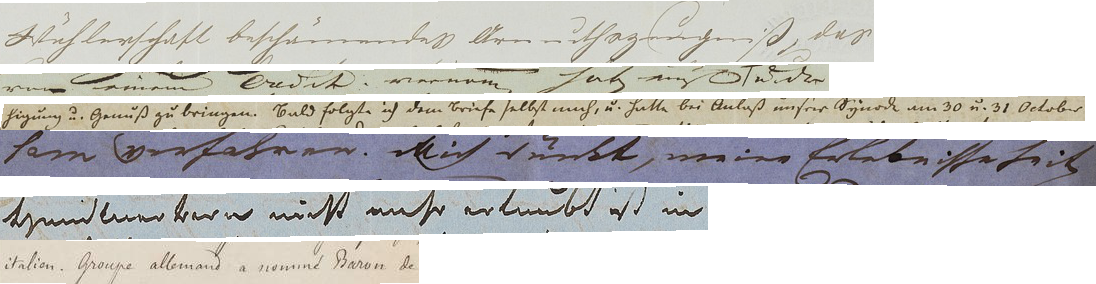
\includegraphics[width=.98\textwidth]{german_lines}
    \caption{Example of lines extracted from the dataset of the ICDAR HTR competition \cite{icdarComp2017}.}
    \label{fig:germanlines}
\end{figure}

%copied from proposal [!]

\section{Computer Assisted Transcription} %TODO, brand corrective/directive

%Due to the limitations of current handwriting recognition methods, we believe that a fully automated handwriting transcription is out of reach with the present of technology. We thus turn our attention to semi-automated recognition approaches, where we are still using a human to transcribe, but also some intelligent recognition technology. A semi-automated solution will outperform a fully automated system in terms of accuracy and is still far more effective than completely manual transcription. 
There tends to be two primary CAT (Computer Assisted Transcription) methodologies: corrective and directive. Corrective CAT methods rely on handwriting recognition to do most of the work, and then users provide feedback correcting some errors of the recognition, where the gain comes from other errors being automatically corrected or being assisted so that corrections are easier to make.

In a directive CAT method, the user provides some of the initial input to the system and it uses this to transcribe more than what the user inputted.
%Standard CAT approaches use human feedback in two ways: to correct or direct. Either the user is correcting automatic transcription in an intelligent way, or to seeding and directing the recognition by labeling/transcribing words.
%Both try two use human input in an intelligent way were more is learned than simply the label/correction given. 
An active learning approach to handwriting transcription is similar to CAT, but is not concerned about achieving human level accuracy, just better accuracy, and thus requires less human involvement~\cite{Serrano2010}. 
%Since we wish to have a system with accuracy comparable to human performance, 
We will focus on CAT approaches.

Toselli et al.~\cite{Toselli2007} have explored the realm of corrective CAT using the idea of user-verified prefixes. They use a fairly standard HMM recognition model as the backbone of their approach, and take advantage of the incremental nature of the Viterbi decoding algorithm. The recognition is done for a line of text and the user corrects the first error. The Viterbi decoding is then run again, but this time using the assumption that everything occurring before the correction is correct, and thus reusing the computation up to that point. They have also explored slight variations of the same approach that enable more fluent user input with a touchpad \cite{Toselli2008}, mouse \cite{Toselli2009}, or multimodal means \cite{Toselli2010}, which speed up the transcription process by allowing more intuitive user interaction (Fig.~\ref{fig:Toselli_multimodalCAT}). Their approach relies on a language model to make corrections on a line when a supervision is made. This means this method cannot be used to effectively transcribe documents containing non-sentence writing, such as tables and lists. Serrano, et al.~also have pursued a similar approach, where the user corrects the \textit{n} words in which the recognition model had the least confidence \cite{Serrano2014}.

\begin{figure}
    \centering
    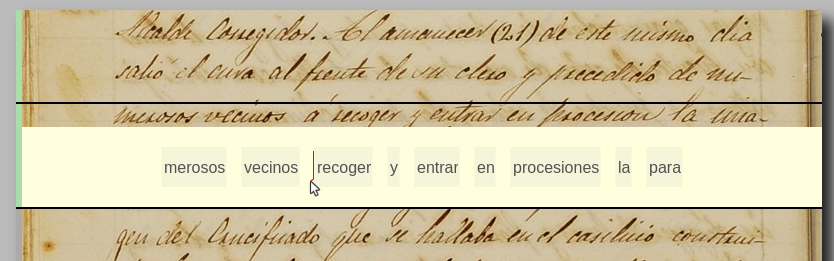
\includegraphics[width=0.95\textwidth]{Toselli_multimodalCAT}
    \caption{A screenshot of a demo of Toselli et al's multimodal CAT system. The red line is drawn by the user to indicate the need to insert a word into the automatically obtained transcription.}
    \label{fig:Toselli_multimodalCAT}
\end{figure}

While it is useful to employ an automatic handwriting recognition method as part of a CAT approach to reduce the human burden, we cannot use the same type of recognition used by these previous CAT systems, where there is a reliance on the predictive capacity of a language model. Some documents are not comprised of only sentences, and thus cannot be transcribed by these methods (e.g.~the name field of census documents, see Figure \ref{fig:ii}). However, many documents are structured such that a pattern can be learned to assist in transcription.


Robert Clawson \cite{Clawson2014}\footnote{You can view a short demo and explanation of his approach at \url{https://www.youtube.com/watch?v=gqdVzEPnBEw}} designed a CAT system for handwritten tabular documents, which have a clear pattern. His approach relies on simply finding matches in the document column of the current word image (red box in Figure \ref{fig:ii}(a). This is essentially query by example word spotting with user oversight. The matched words are assigned the same user-specified label. This provides an accurate CAT system where the user oversees all transcription. The user oversight of matches is accomplished by showing a list of matches to the user (with an adjustable threshold for sensitivity) from which the user removes the false-positive matches. This user interface leverages the human user's natural ability to identify outliers.
Our CAT attempts to also leverage this ability as well.
%However, the approach as a whole is limited as it requires frequent word repetition to be effective. While some tabular documents have this, it is not true for most other documents. Additionally, this method required a computationally expensive preprocessing stage in which a similarity score of all words in a column with all other words in the column had to be computed.
%The word image comparison method used in \cite{Clawson2014} was costly and prohin

\begin{figure}
    \centering
    \begin{subfigure}[t]{0.46\textwidth}
    		\centering
    		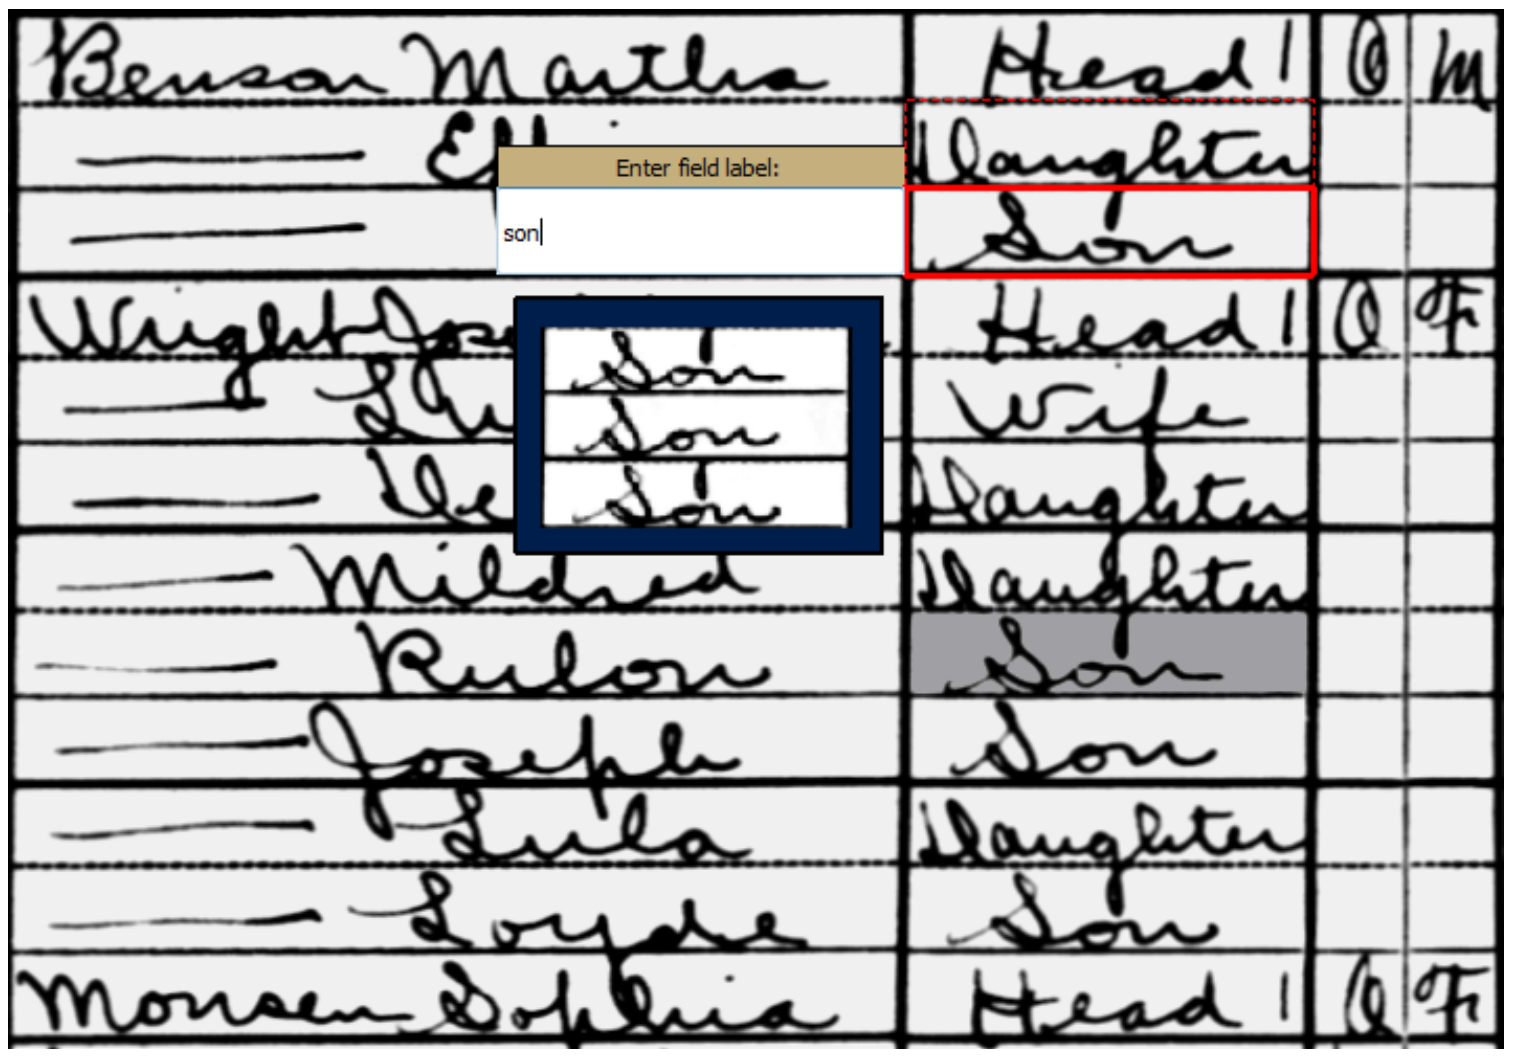
\includegraphics[width=\textwidth]{ii_ex_a}
    		\caption{The red box indicates the current word. A small window shows the matching words that appear elsewhere in the column. The user can get rid of bad matches by either clicking on them or adjusting a  threshold.}
    	\end{subfigure}
    	~
    	\begin{subfigure}[t]{0.46\textwidth}
    		\centering
    		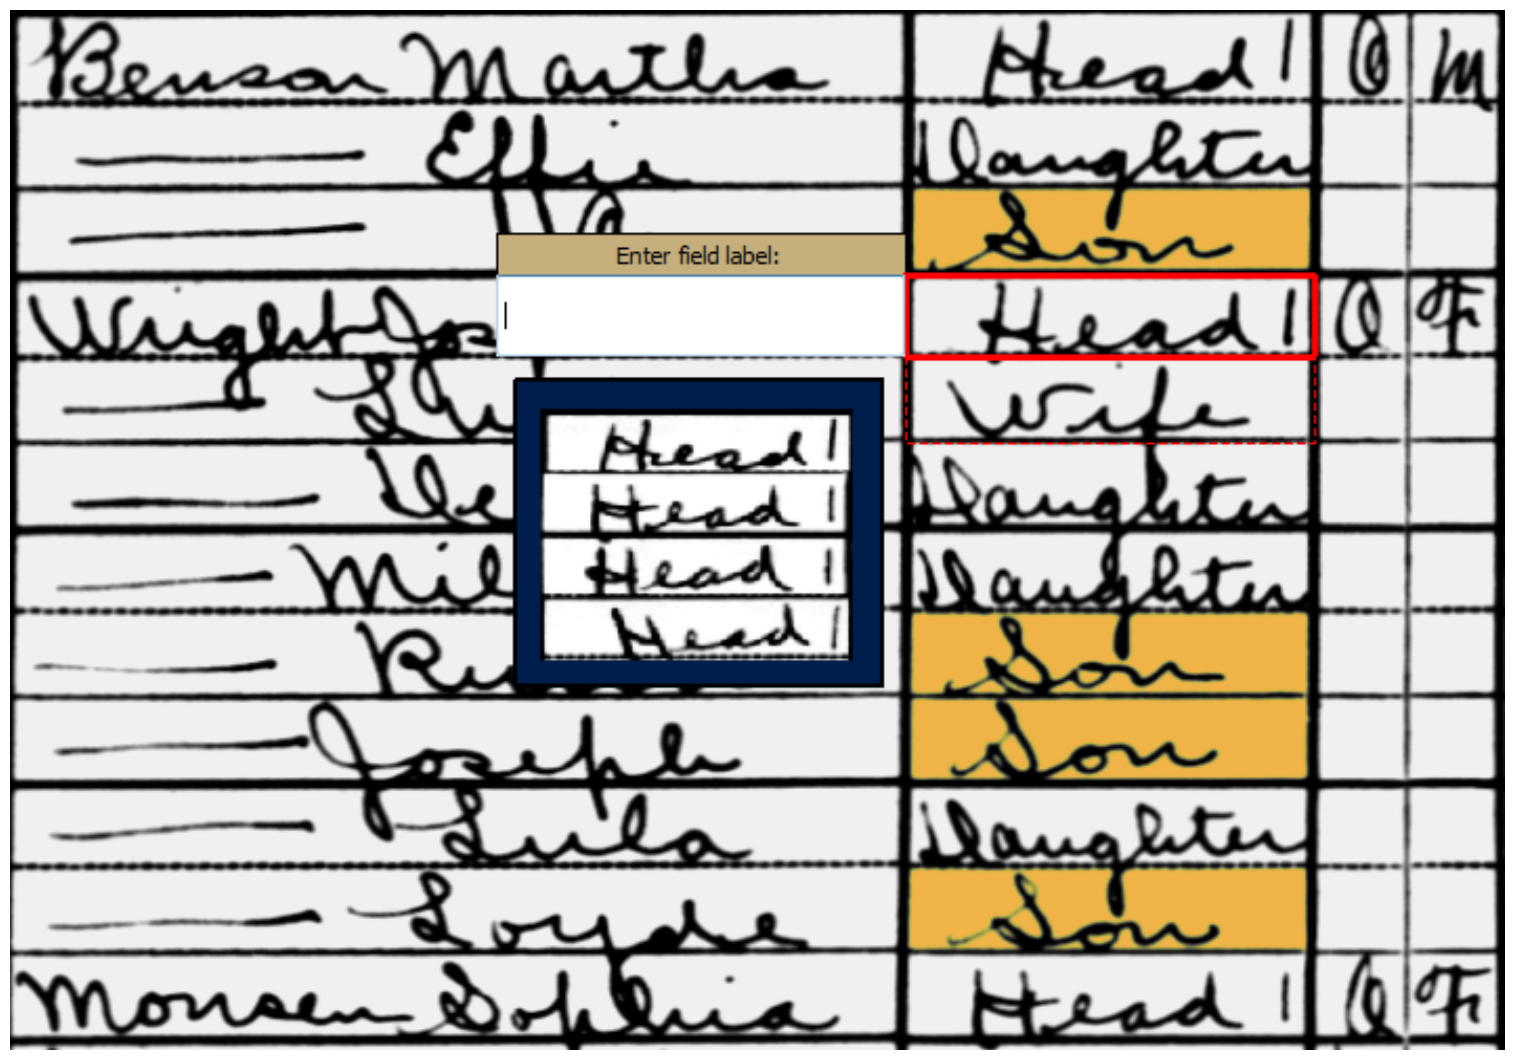
\includegraphics[width=\textwidth]{ii_ex_b}
    		\caption{The matched words, the latter highlighted words, are given the same label when entered.}
    	\end{subfigure}
    	\caption{Clawson's CAT system for tabular documents.}
    	\label{fig:ii}
\end{figure}

%"A Framework for Efficient Transcription of Historical Documents Using Keyword Spotting"
Zagoris et al.~\cite{Zagoris2015} \footnote{A demo of their system is found at \url{http://vc.ee.duth.gr/ws/}} presented a CAT system that was also based on word spotting. In their system when the user is transcribing a word image, they are presented with the results of spotting that image (sorted according to rank). The user can then confirm these spottings by clicking on them, causing them to move to a separate list. When this is done, a relevance feedback loop is activated, which submits another word spotting query of the confirmed image. These spotting results are used to refine the ranked list, providing a better selection. Figure \ref{fig:zagoris} shows a screen-shot of their demo system.
%The description of the system is unclear, but we believe the list of confirmed spottings are then labelled the same as the current word image.
We use the same strategy as \cite{Zagoris2015} to guide the combination of our subword spotting results from multiple queries. Further details are given in Section \ref{combine}.

\begin{figure}
    \centering
    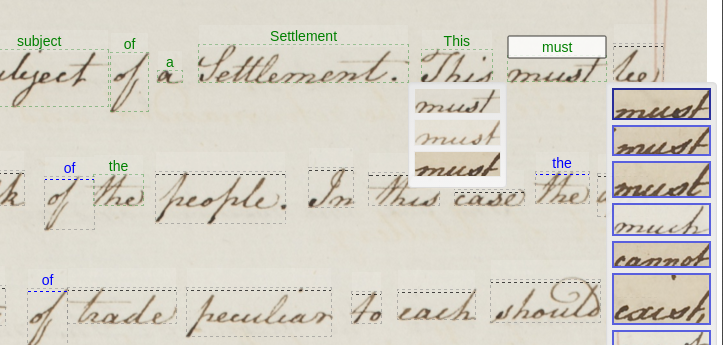
\includegraphics[width=.85\textwidth]{zagoris}
    \caption{A screen-shot of a the CAT system of Zagoris et al.~\cite{Zagoris2015}. The green text indicates hand labeling, the blue text indicates automatic labeling. You can see to the right of the current word (``must'') the current ranked list of spottings (blue boxes).}
    \label{fig:zagoris}
\end{figure}

Neudecker and Tzadok \cite{Neudecker2010} presented a CAT system for historical printed documents that is very similar to the CAT system we present in Chapter \ref{applications}. The system would first segment the individual characters of the documents and run an OCR engine on them. Those characters with low confidence would then be presented to a user for verification in a character session. A single character session contains all the low-confidence character images classified to a single character. An example of their system's character session for the character ``?'' is given in Fig.~\ref{fig:carpet}.  The user merely needs to select the incorrect classifications. Then in a word session, a word image is shown to the user with possible transcriptions for the word, from which they select the correct one. There are three key strengths of this system. One is that as long as the document’s characters can be segmented, it can work. The second is that it formats all user tasks as selections, rather than typing, and they are quickly completed. This creates a much more enjoyable experience for the user. The third key strength is that it is highly parallelizable for crowd-sourced transcribing. This parallelism is achieved because all character sessions are independent of one another and all word sessions are independent of one another. Our system follows this method's pattern so it has flexibility of document types, simple user tasks and a parallelizable framework.

\begin{figure}
    \centering
    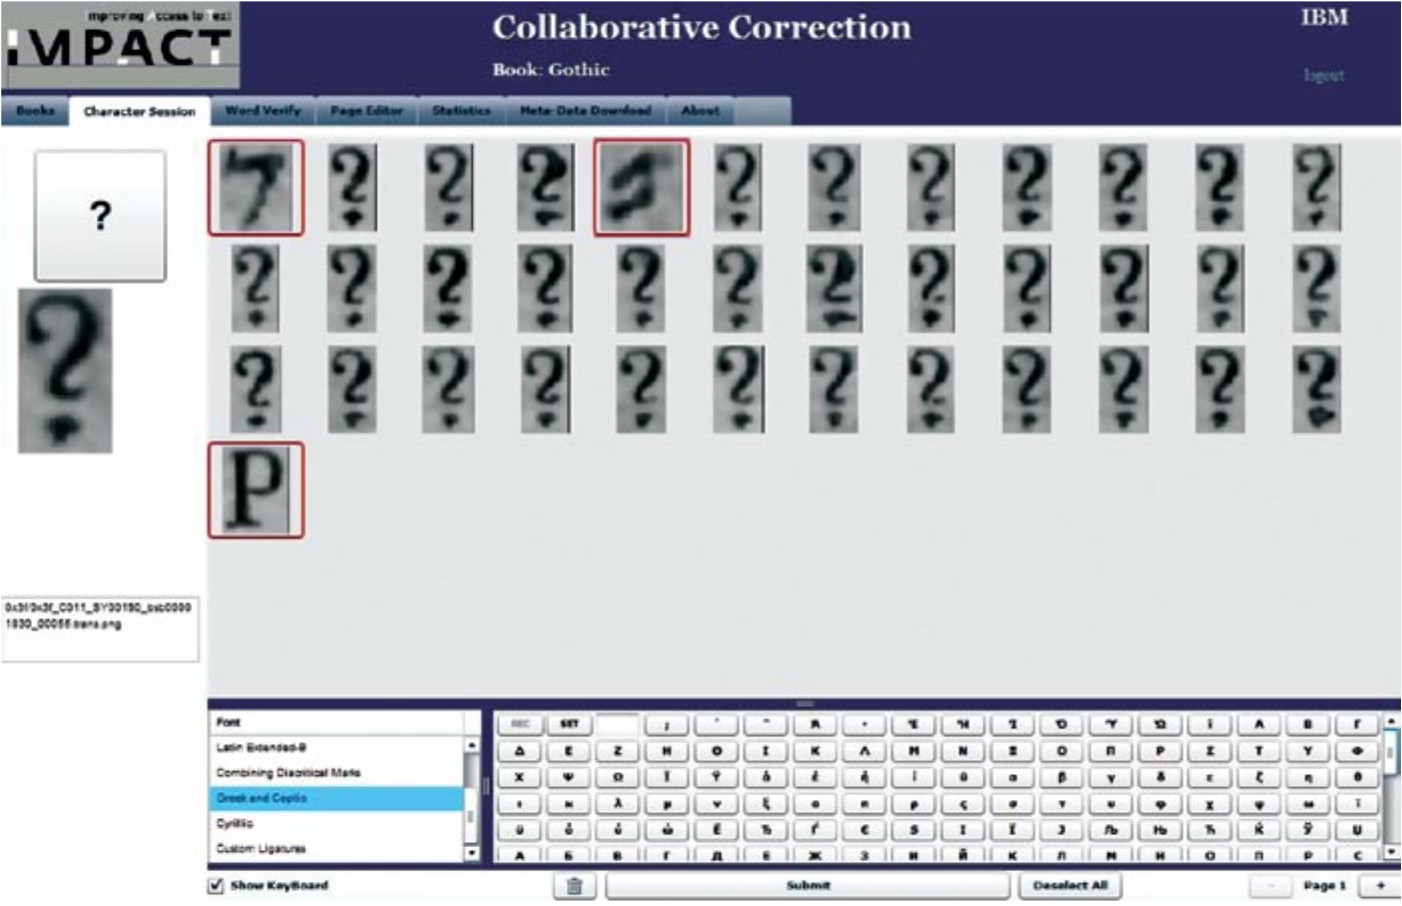
\includegraphics[width=.85\textwidth]{carpet}
    \caption{A screen-shot of a character session for ``?'' from Neudecker and Tzadok's CAT system \cite{Neudecker2010}, taken directly from their report \cite{Neudecker2010}. Notice how easy it is for a user to simply click on the erroneous classifications.}
    \label{fig:carpet}
\end{figure}

Retsinas et al.~\cite{Retsinas2015} expanded on \cite{Neudecker2010} to reduce the amount of user input required by clustering character images together. By viewing an average of a character cluster (where the characters are overlapped), the user can then assign the whole cluster a character label or reject the cluster as being incoherent (i.e.~the cluster contains multiple characters). See Figure \ref{fig:retsinas_ex} for an example. Though requiring more thought from the user, this prevents the tediousness of examining all character images. %Clustering could be applied to our work; it would be more difficult with handwriting, though using online learning to initialize clusters may overcome this. We, however, will not pursue it at this time.
We attempt to use clustering in our own CAT method, however we cannot perform the overlap due to the greater variance in handwriting. Instead we take the approach of \cite{Clawson2014} and simply group clusters together to help visual discrimination.

\begin{figure}
    \centering
    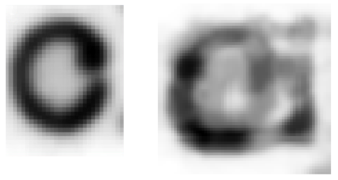
\includegraphics[width=.4\textwidth]{retsinas_ex}
    \caption{Examples of a good cluster (`c') and an incoherent cluster (multiple character classes) taken from \cite{Retsinas2015}.}
    \label{fig:retsinas_ex}
\end{figure}

While we have not seen it done, it would be relatively easy to transfer the results of RNN/CTC-based automatic transcription method to CAT by extracting the top-N transcriptions from the network output. These could then be fed to a user for approval and quick correction for most errors. Given the strength of these automatic methods by themselves, we expect a CAT version of them would outperform the older CAT methods discussed in this section. 



%\section{Other Transcription Assistants}
%TODO

%%%%%%%%%%%%%%%%%%%%%%%%%%%%%%%%%%%%%%%%%%%%%%%%%%%%%%%%%%%%%%%%%%%%%%%%%%%%%%
\chapter{Datasets}\label{datasets}

We use three datasets in our evaluations: the IAM handwriting dataset, the Bentham dataset, and a dataset we extracted from the U.S.~1930 census, which we refer to as Census Names. In this chapter we describe each of these datasets and additionally describe our lexicon.

\section{IAM Dataset}

The IAM handwriting dataset \cite{IAM} is a dataset collected by having human subjects copy certain paragraphs of printed text into handwriting. They were instructed to keep lines well separated and the dataset is very clean as a result. It contains annotations to the word level. We used the provided test set split, the combine training and validation 2 splits as our training set, and the validation 1 set as our validation set.
Example lines from the IAM dataset can be seen in Figure \ref{fig:IAMExamples}.
The test set has 96.1\% of its contents in our lexicon.
These sets have the respective sizes and number of (exclusive) authors:\\
\indent \indent Training: 55106 words, 326 authors\\
\indent \indent Validation: 7089 words, 46 authors\\
\indent \indent Testing: 14600 words, 128 authors

\begin{figure}
    \centering
    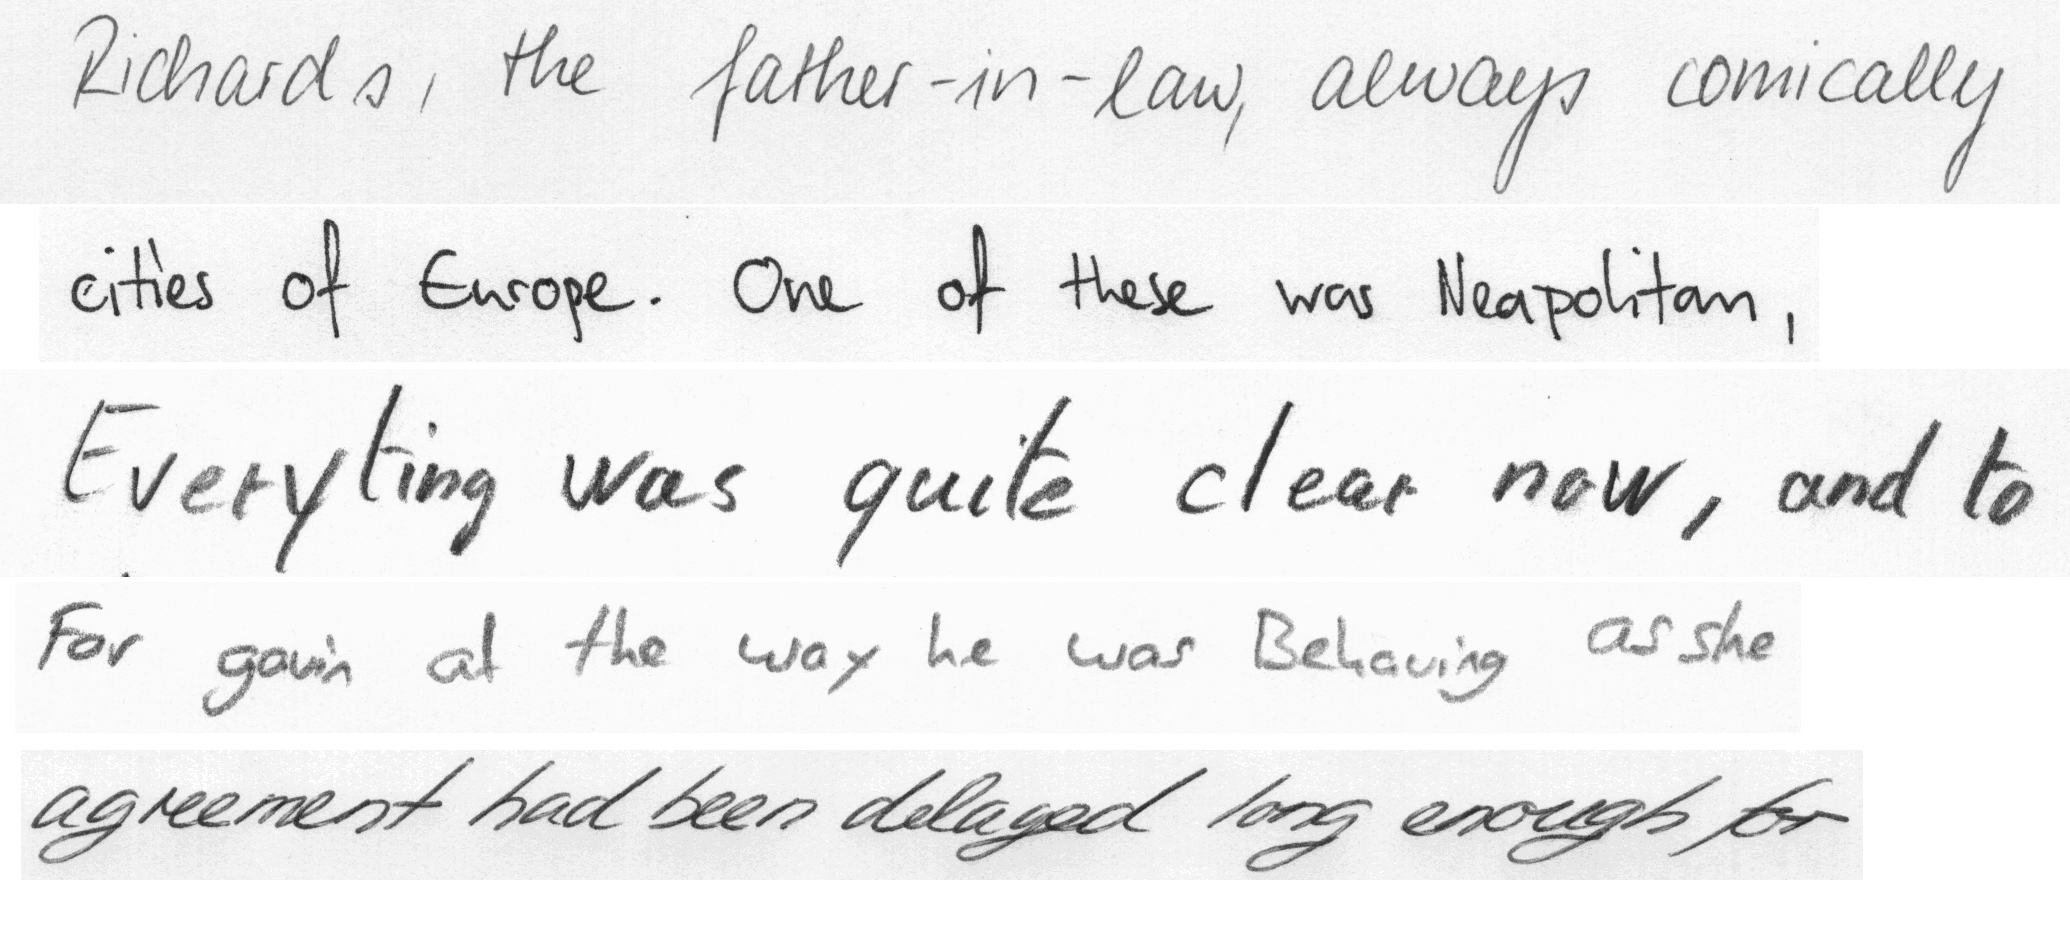
\includegraphics[width=.9\textwidth]{IAM_examples}
    \caption{Examples of lines from the IAM dataset.}
    \label{fig:IAMExamples}
\end{figure}

\section{Bentham Dataset}

The Bentham dataset \cite{bentham} is a collection of documents written by the 17th century philosopher Jeremy Bentham. While there are a plethora of errors we corrected in the ground truth, that ground truth we use differs significantly from that which is officially released, though it is based on it. 
Our training, validation, and test sets are based on the official split, but are not identical.
We ensured pages are exclusive to a single set.
%As we are observing a CAT application of subword spotting it would be optimal that the ``seed'' training set would cover all writing styles. We mix the word instances assigned to the training, validation, and test sets; this likely covers all writing styles and it would be very feasible to randomly label words of a segmented dataset.
Example lines from the Bentham dataset can be seen in Figure \ref{fig:BenthamExamples}.
The test set has 94.9\% of its contents in our lexicon
These sets have the respective sizes:\\
\indent \indent Training: 8490 words\\
\indent \indent Validation: 1071 words\\
\indent \indent Testing: 860 words

\begin{figure}
    \centering
    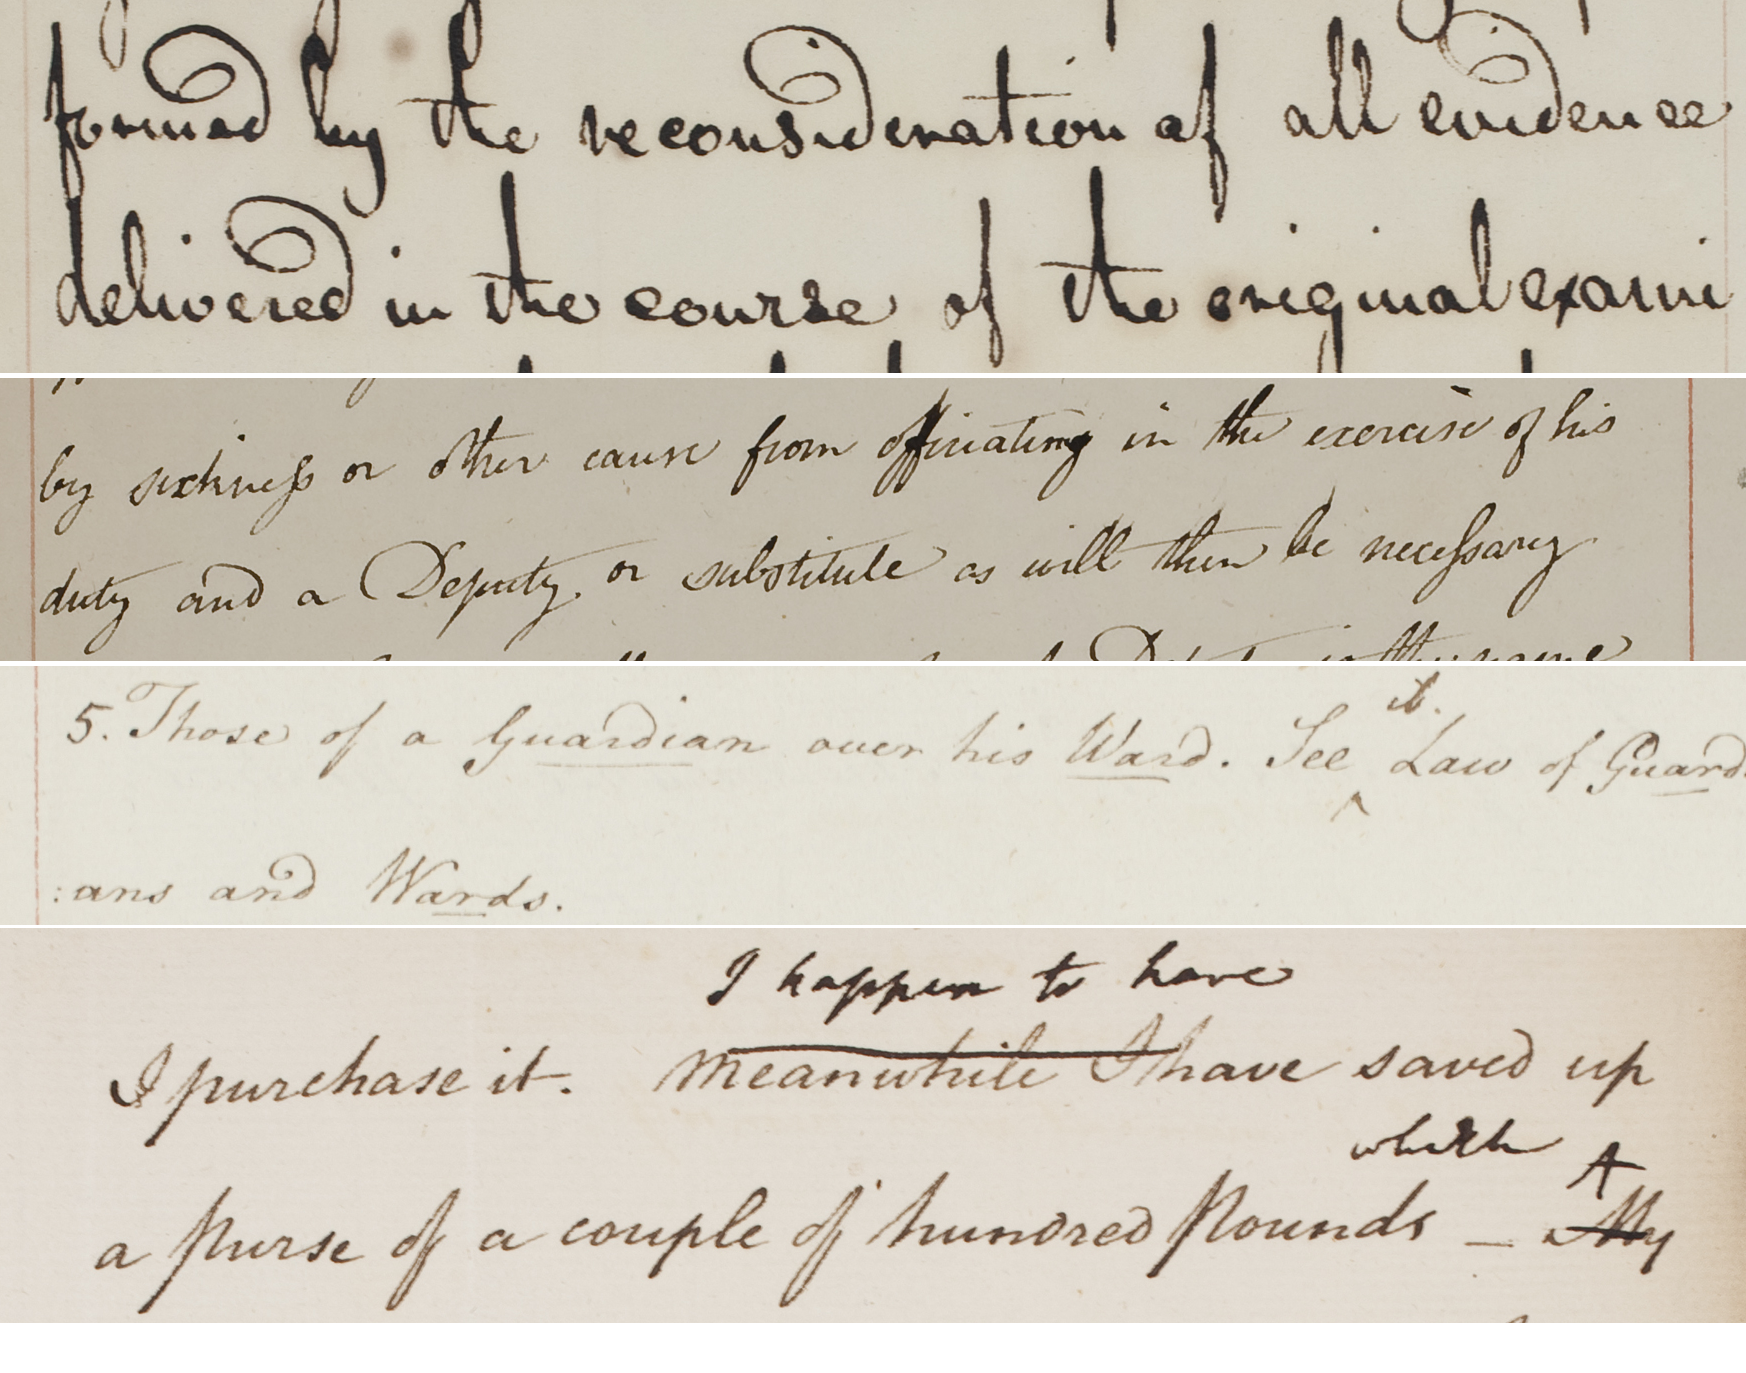
\includegraphics[width=.9\textwidth]{bentham_examples}
    \caption{Excerpts from the Bentham dataset.}
    \label{fig:BenthamExamples}
\end{figure}

\section{Census Names Dataset}

%These files are in py_stuff/census_prep and robert_stuff/document_project/apps_src/field_cropper
The Census Names dataset is an extraction of names from the United Stated of America 1930 census. FamilySearch provided us the ground truth index as well as a  registration of the form images (rotation, scale and offset to align them). We extracted the name fields by first averaging the registered images (Figure \ref{fig:makenames} a) together and manually enhancing the contrast of the resulting image (Figure \ref{fig:makenames} b). We then hand annotated this average image with the lines of the form, using straight lines (Figure \ref{fig:makenames} c). Next we processed each image individually by doing a second registration with the hand annotated form lines by the following. First, we globally moved all the form lines together to maximize the summed inverse pixel intensity (darker is better) along the form lines. This was done by scanning 50 pixels in the four cardinal directions separately (Figure \ref{fig:makenames} d). We then tried all positions in a $7\times 7$ neighborhood around the combined the best x and y positions from the separate horizontal and vertical scans. %(Figure \ref{fig:makenames} f)
 Then, for each individual cell of the form, a small (12 pixel) vertical or horizontal histogram is created around each for the four lines forming the cell boundaries (Figure \ref{fig:makenames} e) and is used to locally snap the cell boundary to the darkest part of the histogram (Figure \ref{fig:makenames} f). This yields a very precise registration in most cases. We then manually segmented the words (last name, first name, middle initial/name) within each cell (Figure \ref{fig:makenames} g). 
Example lines from the Census Names dataset can be seen in Figure \ref{fig:NamesExamples}.
The test set has 83.7\% of its contents in our lexicon
These sets have the respective sizes:\\
\indent \indent Training: 6292 words\\
\indent \indent Validation: 718 words\\
\indent \indent Testing: 2130 words


\begin{figure}
    \centering
    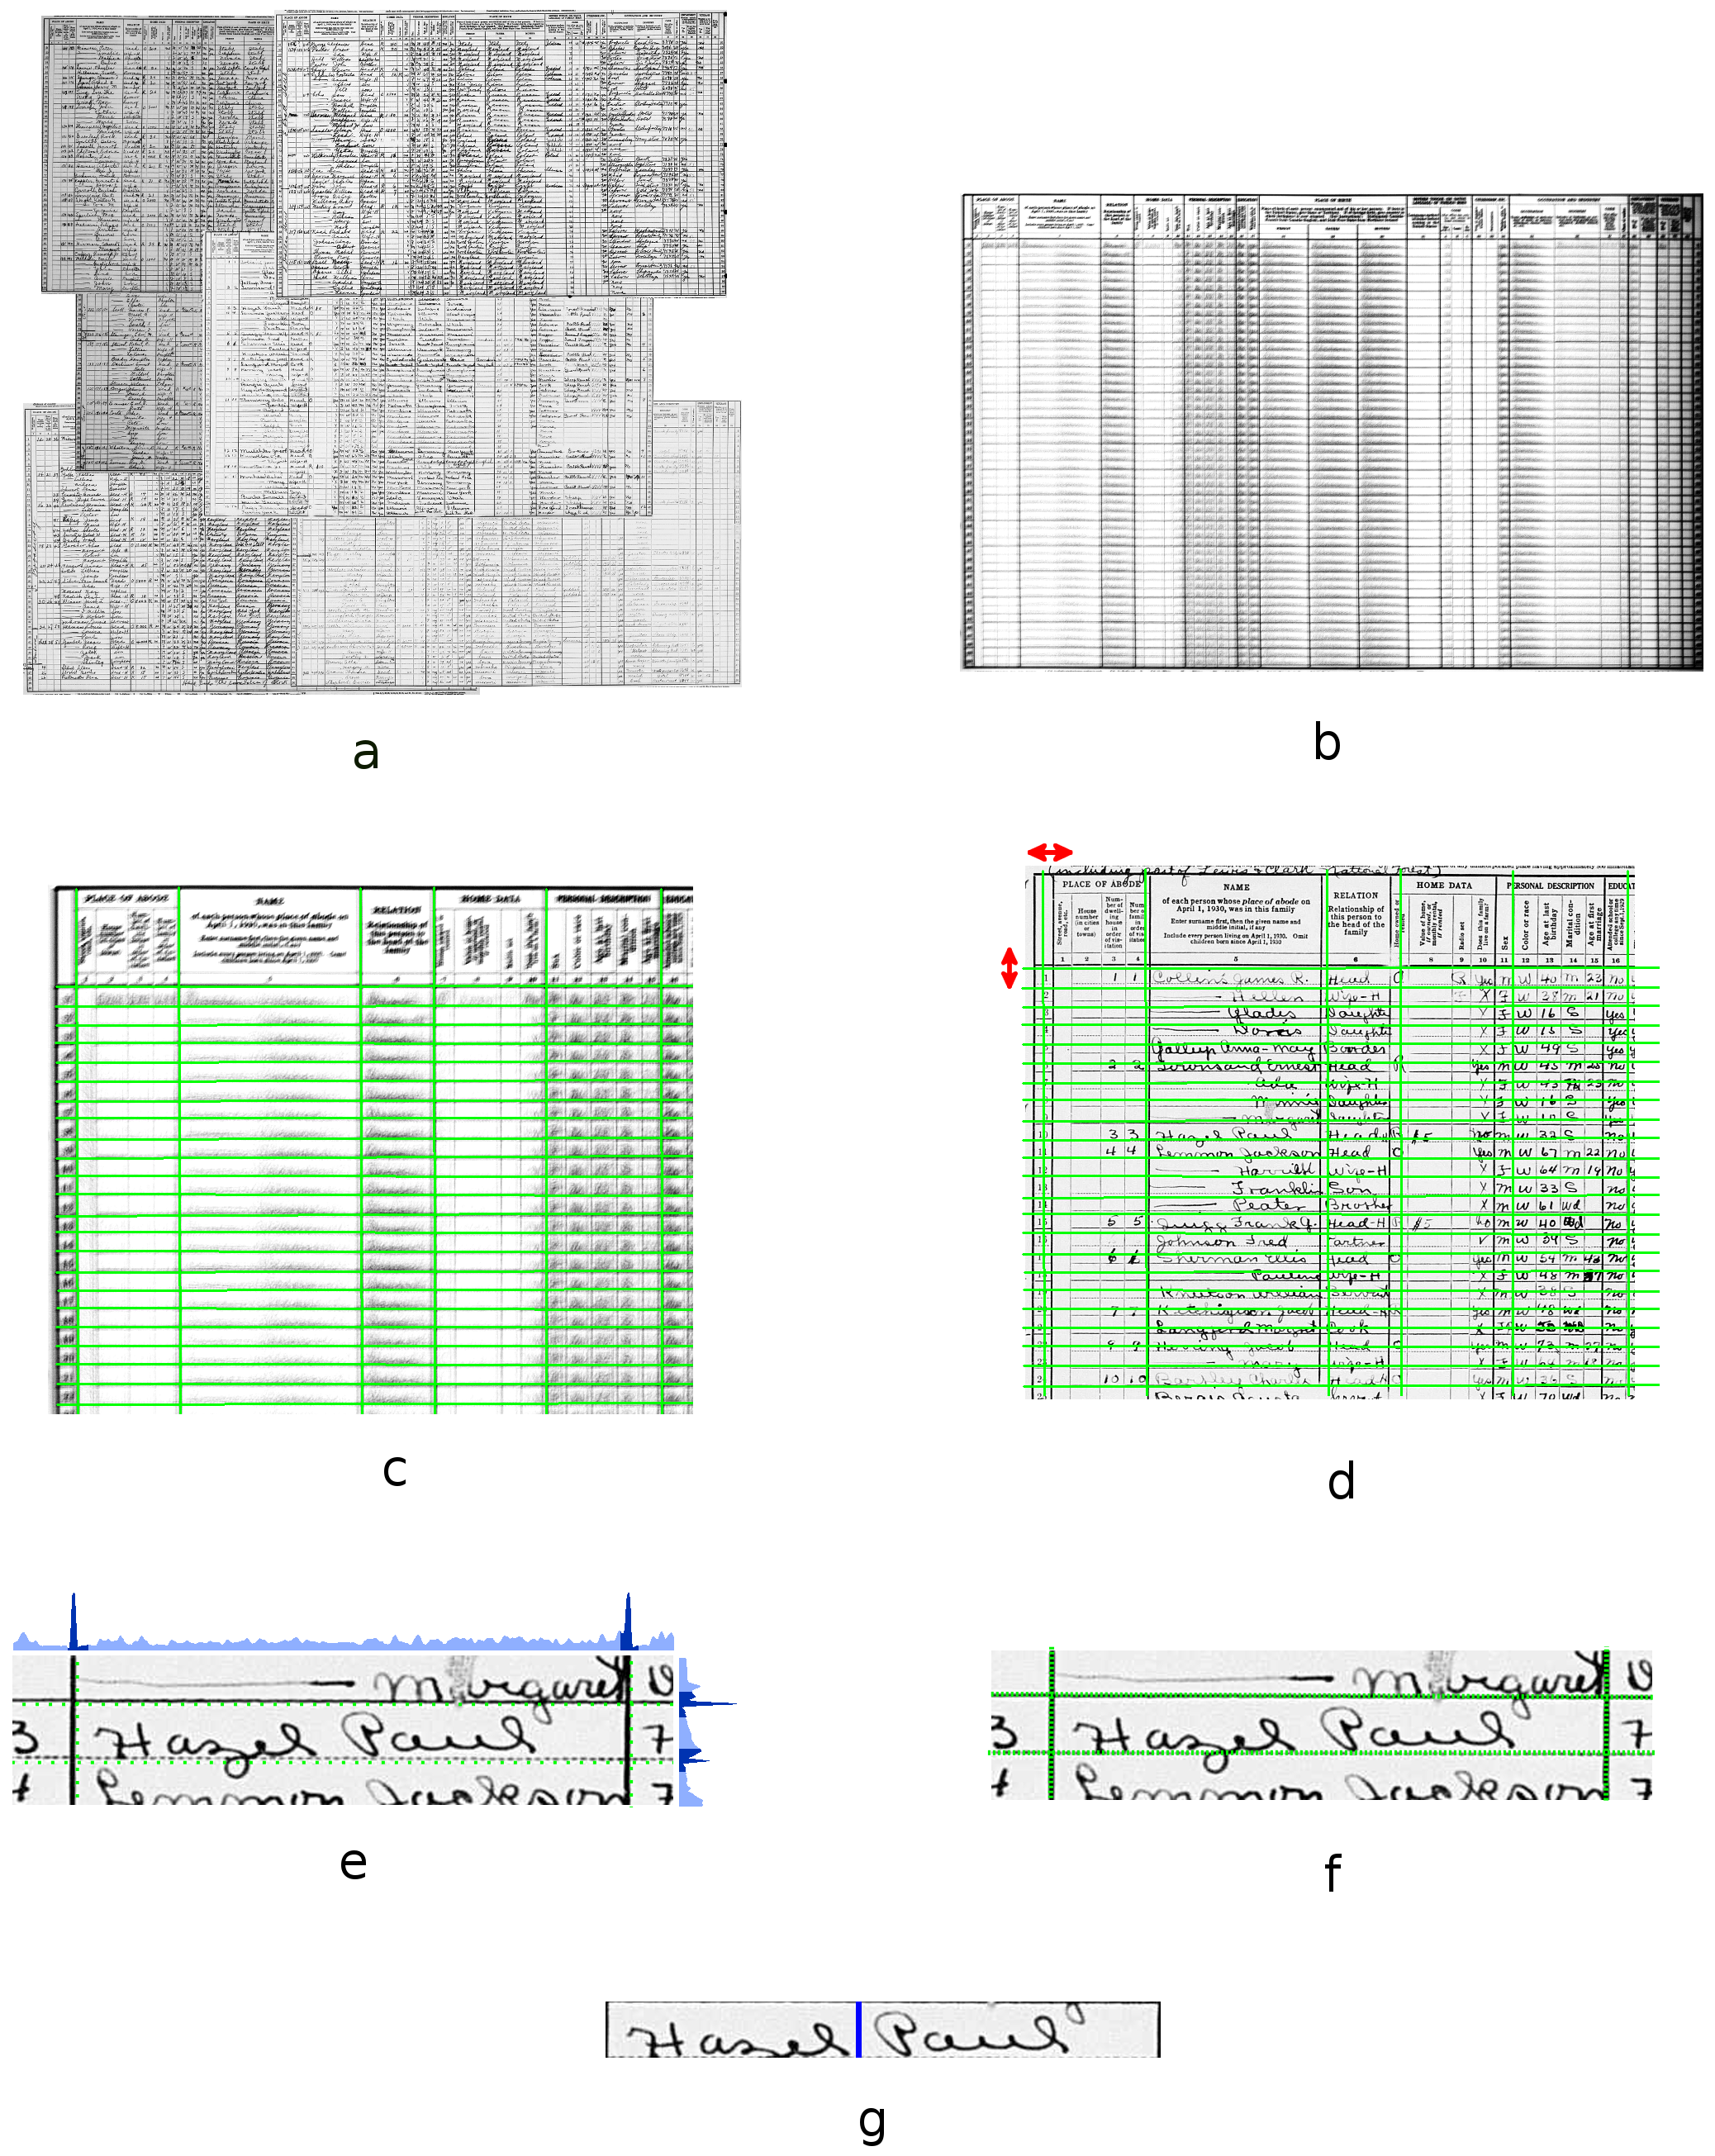
\includegraphics[width=.9\textwidth]{makenames}
    \caption{Process for extracting names from US 1930 census forms for Census Names data set. We begin with registerd forms (a). Then we average the images together (b). The average image is used to mark form boundaries manually (c). The lines are registered to specific census image (d). At each cell a histogram is computed around the cell boundaries (dark blue) (e). The cell boundaries are snapped to the histogram peaks (f). Word boundaries were manually annotated for each cell (g).}
    \label{fig:makenames}
\end{figure}

\begin{figure}
    \centering
    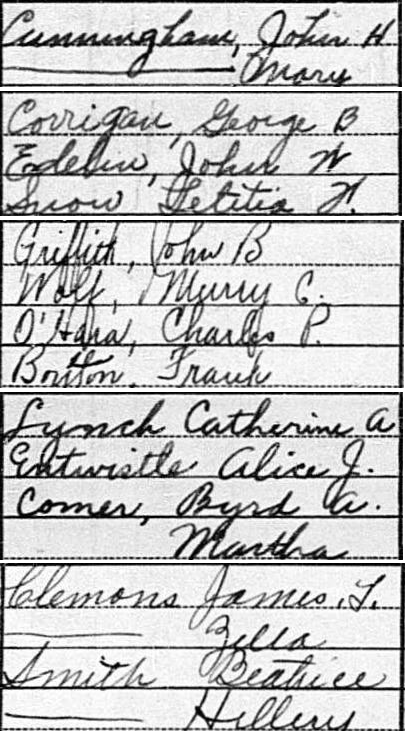
\includegraphics[width=.5\textwidth]{names_examples}
    \caption{Excerpts from the Census Names dataset.}
    \label{fig:NamesExamples}
\end{figure}

\section{Character Annotation}

For the testing portion and a small validation set of the Bentham and Census Names datasets, we produced a character segmentation ground truth. We annotated the word segmentation ground truth by marking the point between characters, meaning character boundaries do not overlap, in addition to a tighter start and end boundary for the word (first and last letters), as seen in Figure \ref{fig:charseg}.

\begin{figure}
    \centering
    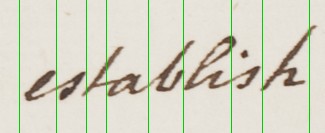
\includegraphics[width=.5\textwidth]{charseg}
    \caption{Example of hand annotated character segmentation.}
    \label{fig:charseg}
\end{figure}

\section{Lexicon}

%Lexicon was created with extractMostFrequentNames.perl
%Merged(intersection) wordsEn.txt with last and first names with 1000 frequency count.
%108,028 words and 6,939 names
%SIL International, linguistics site
For our CAT methods, we require a lexicon. We choose to use a large English lexicon as this would indicate the methods could generalize to other corpi. We obtained a lexicon from SIL International at \url{http://www-01.sil.org/linguistics/wordlists/english/} which contained 108,028 words (not including names). We also desired a large lexicon of names which would enable the Census Names dataset to be transcribed. FamilySearch provided us with data from the US 1940 census, which listed all names appearing in those records along with a count of how many times they occurred. We took all names occuring at least 1000 times, leaving us with a list of 6,939 unique names. Combining these two sets gave us a lexicon size of 114,968. We use the full lexicon for the Bentham dataset, but only the names portion for the Census Names dataset.

%%%%%%%%%%%%%%%%%%%%%%%%%%%%%%%%%%%%%%%%%%%%%%%%%%%%%%%%%%%%%%%%%%%%%%%%%%%%%%
\chapter{Subword Spotting}\label{subwordspotting}
%""
%We implemented multiple CAT systems to provide a well rounded view of transcription through subword spotting. In this chapter we first describe our (sub)word spotting method, then the three CAT systems: transcription through PHOC vectors, transcription through approved subword spottings, and transcription through unassisted subword spotting.

Subword spotting is an extension of traditional word spotting where we allow instances to occur within words. We attempt to localize the spotting in the word to provide additional information. In this work, we focus on small subwords as most applications of subword spotting we explore in Chapter \ref{applications} use these. Figure \ref{fig:explain_sub_spotting} shows an example subword spotting.

In this chapter we describe our implementation of subword spotting and then evaluate many aspects of its performance, including full word, uni-, bi-, and trigram spotting as well as multi-query aggregation.


\section{Implementation}

\subsection{Architecture}

Our subword spotting is built on the segmentation based word spotting method PHOCNet \cite{sudholt2016 sudholt2017} which we converted to perform a sliding window over the word images. \cite{sudholt2017} uses a deep convolutional network trained on word images with pyramidal histogram of characters (PHOC) \cite{Almazan2014} as the target vectors. This method can word spot by both query-by-string (QbS) and query-by-example (QbE), that is querying with text words and word images. See Section \ref{relatedwork_wordspotting} for the details of PHOC vectors. We used a case insensitive PHOC vector and include the bigrams used in \cite{sudholt2016}. We note that the bigrams used in the PHOC vector overlap with, but are not identical with the bigrams we spot; changing this so that they were identical did not improve results. 



Our network architecture varies slightly from \cite{sudholt2017} and is outlined in Figure \ref{fig:network}. We note the reduction in the number of channels in the layer before the temporal pyramid pooling (TPP) and fully connected layers; this is to reduce the size of featurized images (which are saved after this layer).  We used the Caffe framework \cite{caffe}.

%SPP \cite{SPP} is a method of allowing a network with fully connected layers to handle images of arbitrary size. This is accomplished by performing a pooling (max in our implementation) over windows of the image. The first window encompasses the full image and then it proceeds by dividing the windows into 4 at each level down. We use 3 levels for all datasets except the Census Names dataset, which has smaller characters. We use 2 levels for the Census Names dataset to allow the network to operate on smaller images (the SPP won't be creating windows of subpixel size).

TPP is a slight mofication of SPP \cite{SPP}, which is a method of allowing a network with fully connected layers to handle images of arbitrary size. This is accomplished by performing a pooling (max in our implementation) over windows of the image. The first window encompasses the full image and then it proceeds by dividing the windows at each level down. TPP uses the same idea, but only divides windows horizontally as verticle information is not useful once word images are featurized. We use 5 layers (dividing the image into 1, 2, 3, 4, and 5 even windows) for all datasets except the Census Names dataset, which has smaller characters. We use 4 layers for the Census Names dataset to allow the network to operate on smaller images. We additionally modify TPP slightly to handle the corner case of small images such that the windows adjusted to be slightly overlapping at a particular level if a window had no pixels at that level.

\begin{figure}[t]
    \centering
    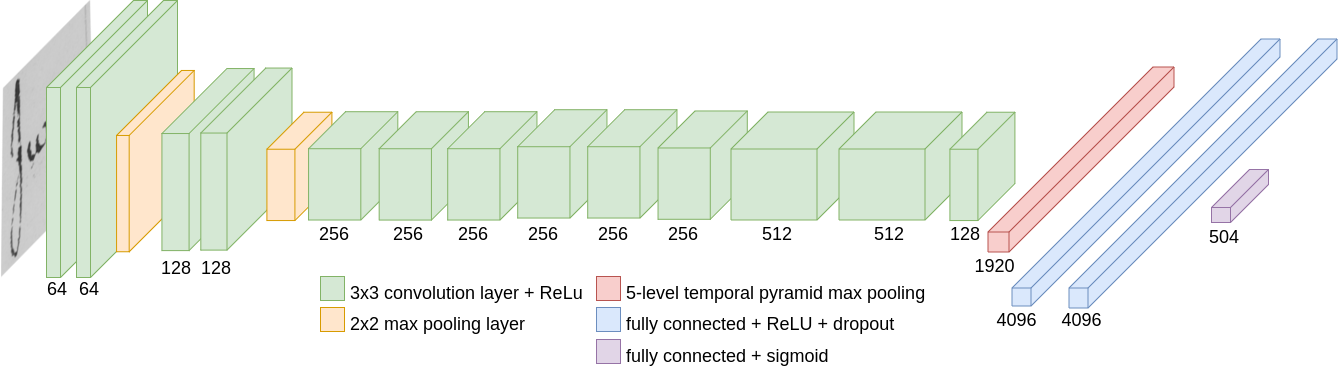
\includegraphics[width=.98\textwidth]{thesis-phocnet}
    \caption{Network architecture for embedding images as PHOC vectors. The numbers beneath each layer represent the number of channels. As the network uses spatial pyramid pooling before the fully connected layers, it can accept images of any size.}
    \label{fig:network}
\end{figure}

\subsection{Training}

In training, we used a batch size of 10, a learning rate of $10^{-4}$, weight decay of 0.00005, and the Adam optimizer \cite{adam}.
%decay the learning rate so that the learning rate at iteration $i$ is $r_i = r_0 (1 + 0.0001 i)^{-0.75}$ (``inv'' policy in Caffe).
We train until out validation loss begins to increase (passes a minimum), indicating overfit.
We then test the validation set MAP for various iterations (including and previous to our stopping point) to find the maximum performance, as MAP generally peaks before the loss reaches its minimum.
%We then begin training with a learning rate of $10^{-5}$ 4000 iterations prior to the MAP peak, stopping again when the validation loss begins to increase. 
%We then repeat the process of finding the validation MAP peak.

During training, we use a distortion augmentation technique similar to the one described in \cite{wigington2017}. In the augmentation technique each example is distorted by placing control points in grid fashion on the image and then distorting the image by perturbing these control points. This is repeated at finer scales; the control points are more closely aligned and the perturbations smaller. See Figure \ref{fig:augmentation} to see the result of this augmentation on a word image. This augmentation greatly reduces possible overfitting during training as the network never sees the exact same images twice.
%For the Bentham dataset we started with control points $d^0_{control} = 64$ pixels apart and initial perturbations with a standard deviation of $\sigma^0_{control} = 0.3 d^0_{control}$. We decreased control point distance by a factor of 0.5 and decreased the perturbation standard deviation by a factor of 0.6 for each of 4 levels, so that if $l$ is the level, $d^l_{control} = 64(0.5^{l})$ and $\sigma^l_{control} = 0.3 d^l_{control} (0.6^{l})$.
For the Bentham dataset we started with control points $d_0 = 64$ pixels apart and initial perturbations with a standard deviation of $\sigma_0 = 0.3 d_0$. We decreased control point distance by a factor of 0.5 and decreased the perturbation standard deviation by a factor of 0.6 for each of 4 levels, so that if $l$ is the level, $d_l = 64(0.5^{l})$ and $\sigma_l = 0.3 d_l (0.6^{l})$.
Similar to \cite{sudholt2016} we balance word counts in the training set. However, we allow far more instances of each word (more duplicates of images) in the training set due to our improved augmentation technique. We set a goal for the count of each word of $c_{goal} = 0.6c_{max}+0.4c_{mean}$, where $c_{max}$ is the maximum count of any word and $c_{mean}$ is the mean count of all words ($c_{max}$ is capped at 200 to prevent too large of training sets). A set of $c_{goal}$ instances of each word form the training set, including some duplicates when needed.

Each word image is a unique size, however, to train on a GPU all instances in a batch must be the same size. We circumvent this by resizing all word images in a batch to the same size. The height and width composing this size are drawn from Gaussian distributions parametrized by the mean of the height and width of
the word images of the batch, the standard deviations being $2/3$ the standard deviation of the height and width of the batch images. This is additionally capped at a maximum and minimum height (X,X) and width (X,X).

We used a validation set to determine the optimal number of training iterations by observing when QbS word spotting on the validations set peaked in performance.

%NOT TRUE ANY MORE? not in training at least
%To prevent images too small for the network (SPP layer is sensitive to this), any instances smaller than 32 pixels in their smallest dimension are resampled with a larger bounding box. Additionally 
We scale any images taller than 200 pixels to be 200 pixels tall; this improves efficiency and provides some normalization to the titles found in the Bentham dataset.

\begin{figure}
    \centering
    \begin{subfigure}[t]{0.46\textwidth}
    		\centering
    		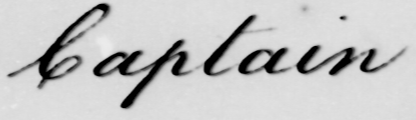
\includegraphics[width=\textwidth]{Captain_unwarped}
    		\caption{Unwarped image.}
    	\end{subfigure}
    	~
    	\begin{subfigure}[t]{0.46\textwidth}
    		\centering
    		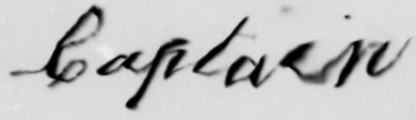
\includegraphics[width=\textwidth]{Captain_warped}
    		\caption{Image warped using augmentation technique from \cite{wigington2017}.}
    	\end{subfigure}
    	\caption{Example of data augmentation used in training.}
    	\label{fig:augmentation}
\end{figure}

\subsection{Determining Window Widths}\label{detirminewindowsize}
Because the neural network takes in some context, it is difficult to measure what the optimal sliding window size should be based on visual width.
Additionally each n-gram is likely to have a different optimal window size. We determine the optimal window size for each n-gram as follows.
We first compute the MAP for a range of window sizes (stepping 4 pixels), smoothing these results and taking the max. We smooth by averaging a window of 3 steps (average MAP from 3 window sizes), using 2 steps on the edges. For efficiency we cluster all the resulting window sizes (from each n-gram) into 10 clusters using k-means, assigning each n-gram the cluster mean as its width. This allows us to pre-compute PHOC vectors of only 10 window sizes.% for all n-gram.

\subsection{Running}

To prepare for spotting, we save the output of the network up to the spatial pyramid pooling as a featurization of each word image. Then subwindows of this featurization can be passed to the latter part of the network (starting with spatial pyramid pooling) to generate a PHOC vector. As part of the preprocessing we extract PHOC vectors for subwindows with a stride of 4 pixels (step of 1 in the featurized image as the network reduces images by a factor of 4) for the 10 sizes determined using the method in the previous section.

%the number of characters being spotted and an estimated character width for the dataset; 37? 33 pixels for the Bentham dataset, 20 for the Census Names dataset.
%This preprocessing allows us to forgo running the network as we merely need

%For performing QbS, one compares the PHOC vector representing the query word or n-gram to the output of the network. For QbE, the outputs of the network are compared against eachother.
\cite{sudholt2016} used the Bray-Curtis dissimilarity to compare PHOC vectors (both string and network generated) and we follow the same procedure.
%, however, we found a dot-product similarity, normalizing network outputs, worked better for our implementation.
%The score for a subwindow is the normalized dot product between the query PHOC vector (the network output of the query image or the actual PHOC vector of the query word) and the network's generated PHOC vector for that subwindow.
To reduce computation, we only return the top two highest scored subwindows of a word image which are at least 40\% of the estimated character width apart. Here, we assume an n-gram never occurs more than twice in a word, which is a reasonable assumption for English.


We tried refining top scoring subwindows by slightly adjusting their boundaries and re-scoring, however, we did not see a significant improvement. %and the computation cost was prohibitive (as the featurization of the refined subwindows was not precomputed).

\subsection{Combining QbE Results}\label{combine}

We perform iterative aggregation of QbE results by merging results from consecutive queries. To do this we check for potential overlapping spottings, if there is an overlap (of at least 20\%) we discard the result with the worse/higher score. This, merging by taking the better score, follows what \cite{Zagoris2015} found to be most effective when combining full word spotting results. As further justification, one can think of each n-gram or word as having several prototypical ways it can appear (e.g.~an `a' appearing with or without the tail on top, `\textsf{a}' or `{\fontfamily{qag}\selectfont\footnotesize a}'). By selecting the best/minimum score you select the score computed on the exemplar image with the prototype closest to the instance of interest's prototype.

In the following section we show results of this network's performance on unigrams, bigrams, trigrams and whole words.

%%%%

\section{Analysis of Subword Spotting}

In this section we present results of testing the subword spotting method described above.
%We present our own results of testing the subword spotting method described in Chapter \ref{subwordspotting}. 
As a baseline, we show our network's performance on full word spotting. We evaluate subword spotting unigrams, bigrams and trigrams against our testing portions of the Bentham dataset and Census Names dataset. 

\subsection{Full Word Spotting}

Full word spotting is performed as described in \cite{sudholt2016}, where the neural network is used to generate a PHOC vector of each word image in the corpus. For QbS, each word (string) in the corpus's PHOC representation is used as a query. For QbE, each image which has at least one of image with the same label is used as a query. We compare using mean average precision (MAP). Our results are shown in Table \ref{tab:wordspottingresults} for the Bentham dataset, the Census Names dataset, and, for comparison with PHOCNet \cite{sudholt2016,sudholt2017}, the IAM dataset.

\begin{table}
\centering
\begin{tabular}{| l | c  c | c c | c c |}
  \hline
   & \multicolumn{2}{c|}{IAM} & \multicolumn{2}{c|}{Bentham} & \multicolumn{2}{c|}{Census Names}\\
  Method & QbS & QbE & QbS & QbE & QbS & QbE\\
  \hline		
  %Old network & 0.755 & 0.683 & 0.762 & 0.811 & 0.525 & 0.511  %results with msfNoLRN/sig-bray IAM:208000  BEN:160000 NAMES(less):144000
  Our network  &  0.X & 0.X  &  0.772 & 0.796  &  0.559 & 0.561  %results with new_phocnet(TPP) IAM:X  BEN:X NAMES(less):fine37000
  %bentham:ben_fixed_corpus.gtp
  \\
  PHOCNet\cite{sudholt2016} & 0.830 & 0.725 & - & - & - & - \\
  TPP-PHOCNet\cite{sudholt2017} & 0.934 & 0.827 & - & - & - & - \\
  %? & X & X & X & X \\
  \hline  
\end{tabular}
\caption{MAP for full word spotting results, reported for both query-by-string (QbS) and query-by-example (QbE). Results on Census Names uses network with SPP depth of 2 instead of 3. Using 3 yields QbS:0.525 and QbE:0.511.}
\label{tab:wordspottingresults}
\end{table}
%fixed_corpus QbS: 0.592938 QbE mAP: 0.749275
%,this is with Bray-Curtis QbS mAP: 0.32189  QbE mAP: 0.642274
%cattss_c_corpus QbS mAP: 0.582461   QbE mAP: 0.720274
%nn_valid QbS mAP: 0.79995  QbE mAP: 0.922255
%nn_gwnb_valid QbS mAP: 0.807672  QbE mAP: 0.914204
%Did we overfit to our validation set? Possibly nn_valid has some of nn_gwnb_train
%we trained on nn_gwnb_train (?),
%retraining on nn_train

%cattss_c_train QbS mAP: 0.76686  QbE mAP: 0.822692

%Trying with sigmoind+bray-curtis ...

We first note that our model significantly under performs \cite{sudholt2016} on the IAM dataset (by 7.5\% on QbS and 4.2\% on QbE). We were unable to reproduce their results, mimicking their model, and the architecture changes we make we expected would have a negative effect on performance. It is likely a better word spotting model could be produced, but this was not the the focus of our work.
It is clear that the Census Names dataset is significantly more challenging than the other datasets, however, having above 50\% MAP indicates the network is learning the task to some degree.

\subsection{Subword Spotting}

We use our sliding window method to evaluate spotting uni-, bi- and trigrams on the Betham dataset. We used our ground truth for the testing portion of the Bentham and Census Names datasets which have character boundaries. We considered a spotting to be correct if its window overlapped with the desired n-gram's boundaries by 0.5 of the largest of the two's boundaries and there were no other spottings overlapping with the n-gram more. 
We spotted each letter of the alphabet, the 100 most frequent bigrams (in the English language), and the 300 most frequent trigrams. Each of these n-grams were spotted using QbS, if there was at least one instance of it in the testing set, and all examples of these n-grams in the dataset was used as a QbE query, if there are at least two instances of the n-gram.
Results can be seen in Table \ref{tab:subwordspotting}.
Some qualitative results are show in Figure \ref{TODO}. several (3) n-grams on several words, colored boxes, 1,2,3 seperate. 3 words which share high activations for 3 ngrams
%We show QbS results for both using all n-grams (full) and those n-grams used for QbE (same).

%Effect of window size %TODO
In section \ref{detirminewindowsize} we explained how we found the window sizes we used. We show in Figure \ref{fig:windowsizes} the effect of changing the window size for some selected n-grams.


%Trigrams, having the most context, perform the best by a wide margin. Bigrams and unigrams have very comparable performance. Consistently QbS outperforms QbE, we expect this is because the learned representations of the n-grams (used in QbS) are more invariant than individual n-gram instances, which can have large variation in their context and form.

%fawkes...BENTAN/outUni [Bi,Tri] has top 15 spottings

\begin{table}
\centering
\begin{tabular}{| l | c c c c | c c c c |}
  \hline
   %& \multicolumn{2}{c|}{Bentham} & \multicolumn{2}{c|}{Census Names}\\
   %& QbS & QbE & QbS & QbE \\
   & \multicolumn{4}{c|}{Bentham} & \multicolumn{4}{c|}{Census Names}\\
   &     & weighted & n-gram & instance &     & weighted & n-gram & instance \\
   & QbS & QbS      & QbE    & QbE      & QbS & QbS      & QbE    & QbE \\
  %vvv FIXED vvvv
  \hline %FIX(sig-bray-curtis precomp) NoLRN, 0.5 thresh, 160000 full QbS  same set,  (Bray-Curtis turned on...), NAMES with less-SPP
  Unigram & 0.460 & X & X & 0.395  & 0.316 & 0.439 & 0.188 & 0.280\\ %these are all running (corpus_original.txt)
  Bigram  & 0.541 & X & X & 0.435  & 0.296 & 0.387 & 0.185 & 0.246\\ 
  Trigram & 0.481 & X & X & 0.444  & 0.204 & 0.271 & 0.121 & 0.212\\ 
  \hline %FIX(sig-bray-curtis precomp) NoLRN custom widths, 0.5 thresh, full QbS  same set,  (Bray-Curtis turned on...), NAMES with less-SPP
  Unigram & 0.496 & 0.577 & 0.320 & 0.382  & 0.335 & 0.438 & 0.183 & 0.274\\
  Bigram  & 0.567 & 0.632 & 0.363 & 0.431  & 0.280 & 0.375 & 0.169 & 0.223\\ 
  Trigram & 0.496 & 0.572 & 0.350 & 0.441  & 0.191 & 0.262 & 0.112 & 0.204\\ 
  \hline %new phocnet
  Unigram &  0.X & 0.X & 0.X & 0.X  & 0.X & 0.X & 0.X & 0.X \\
  Bigram  &  0.X & 0.X & 0.X & 0.X  & 0.X & 0.X & 0.X & 0.X \\
  Trigram &  0.X & 0.X & 0.X & 0.X  & 0.X & 0.X & 0.X & 0.X \\
  \hline 
\end{tabular}
\caption{MAP for subword spotting results on the Bentham and Census Names datasets, reported for query-by-string (QbS), QbS weighted by n-gram frequency, query-by-example (QbE) by n-gram (comparable to QbS), and QbE by instance (comparable to weighed QbS).}
\label{tab:subwordspotting}
\end{table}

We notice in Table \ref{tab:subwordspotting} that trigrams have a worse performance compared to bigrams on the Bentham dataset, and on the Census names, unigrams out perform bigrams and trigrams. This immediately seems counterintuitive, as trigrams and bigrams have more context than unigrams. However, n-grams which occur less frequently tend to produce greater error, and the higher n is, the less the n-gram occurs. 
This is demonstrated in Figure \ref{fig:remove}, where n-grams which occur infrequently are removed from our testing set and the MAP increases. This is potentially because there are less examples seen in training (training is balanced at a word, not n-gram, level).


\begin{figure}
    \centering
    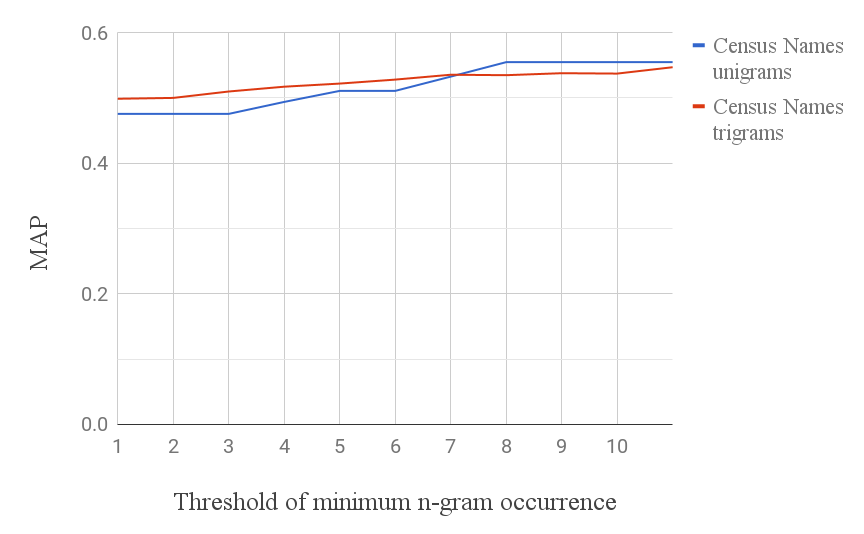
\includegraphics[width=.75\textwidth]{removengrams}
    \caption{MAP for QbS subword spotting results on the Bentham and Census Names datasets, where we only use n-grams in our query set which have an occurrence count above a threshold (in the testing sets). MAP increases, demonstrating less frequent n-grams are more difficult. Only trigrams are shown for the Bentham dataset due to the high frequency of all unigrams and bigrams.}
    \label{fig:remove}
\end{figure}

In Tables \ref{fig:unigram}, \ref{fig:??}, and \ref{fig:??} we show the (M)AP for each n-gram individually. 
%TODO Change to figures
\begin{table}
\centering
\begin{tabular}{| r | c c | c c |}
  \hline
  & \multicolumn{2}{c|}{Bentham} & \multicolumn{2}{c|}{Census Names}\\
  \hline
  unigram & QbS & QbE & QbS & QbE\\
  \hline 
  a & X & X  &   X & X\\
  ...\\
  \hline 
\end{tabular}
\caption{AP for QbS and QbE on each unigram.}
\label{tab:unigram}
\end{table}

%~/caffe/scripts/cnnspp_spotter/cnnspp_spotter models/phocnet_msfNoLRN_featurizer.prototxt models/phocnet_less_embedderSig.prototxt  net/phocnet_lessNoLRN_iter_144000.caffemodel 1 0.25 ./seg_names_corpus_mod.gtp NAME_COLUMNS/ customWidths.txt manual_segmentations_train_val.csv = ../alphabet.txt ../top100_bigrams_in_freq_order.txt ../top300_trigrams_in_freq_order.txt
%~/caffe/scripts/cnnspp_spotter/cnnspp_spotter models/phocnet_msfNoLRN_featurizer.prototxt models/phocnet_msf_embedderSig.prototxt net/phocnet_msfNoLRN_iter_160000.caffemodel 2 0.25 ben_fixed_corpus.gtp page_images/ customWidths.txt manual_segmentations ! ../alphabet.txt 50 1 1 > respotUni_oct10.txt

\subsection{Respotting Subwords}

We had hoped to use approved spottings as new exemplars for an iterative CAT system. To verify the validity of this approach we created an experiment where we continually refine spotting results by spotting with new exemplars and merging the results (see Section \ref{combine}). We show the MAP at each iteration out to 50 iterations in Figures \ref{fig:unigram_respot}, \ref{fig:bigram_respot}, and \ref{fig:trigram_respot}, for uni-, bi-, and trigrams respectively. The first exemplar for an n-gram was selected as the middle score of positive instances from a QbS spotting. The following exemplars were the middle score of the previous QbE spotting's positive instances. We choose to do this as there is a variety of qualities of exemplar images. Taking the middle score should roughly give us a middle quality. The overall quality of MAP is higher in these experiments as we pruned all n-grams which occur less than 100 times, which tend to be the more difficult instances.
We can see that the iterative refinement leads to better results compared to the average of all the QbE scores. It appears that aggregating multiple queries tends to stabilized the bad queries, though it does not out perform QbS (except with trigrams) or individual good QbE queries (as the spikes in performance are not at the end).

\begin{figure}
    \centering
    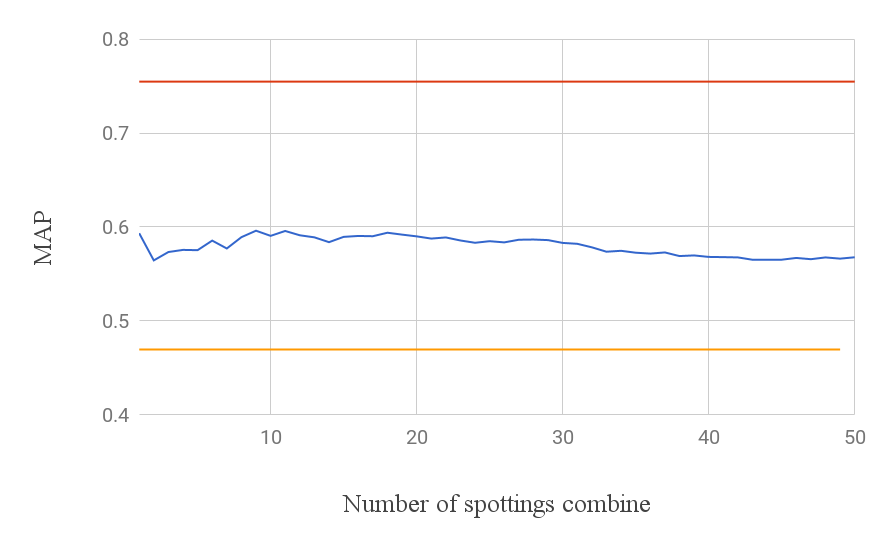
\includegraphics[width=.75\textwidth]{unigram_respot_chart}
    \caption{Unigram MAP when spotting results of consecutive image queries are combine (blue). The red line represents QbS performance and the yellow the average performance of all 50 QbE queries.}
    \label{fig:unigram_respot}
\end{figure}
\begin{figure}
    \centering
    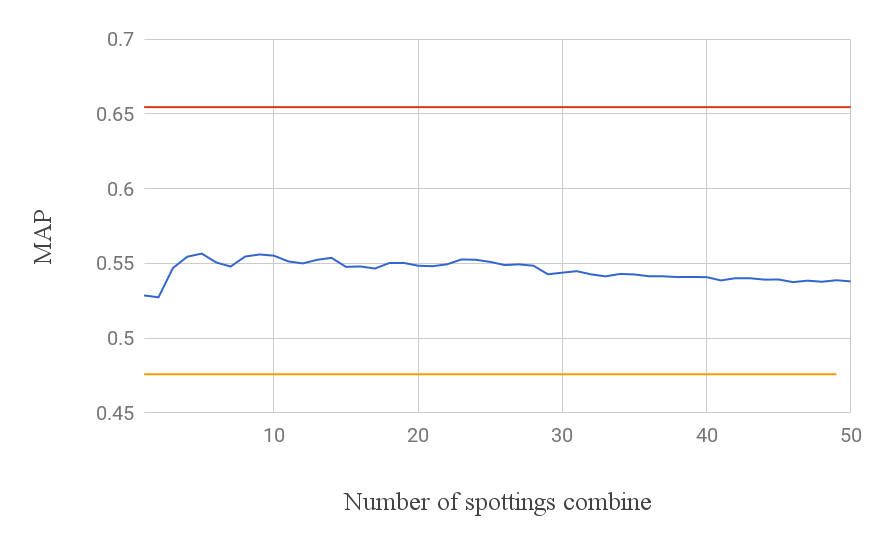
\includegraphics[width=.75\textwidth]{bigram_respot_chart}
    \caption{Bigram MAP when spotting results of consecutive image queries are combine (blue). The red line represents QbS performance and the yellow the average performance of all 50 QbE queries.}
    \label{fig:bigram_respot}
\end{figure}
\begin{figure}
    \centering
    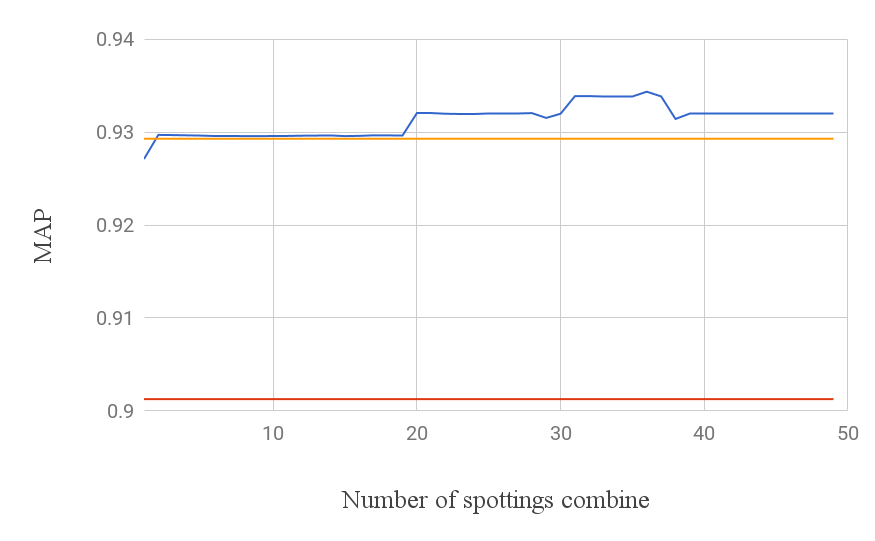
\includegraphics[width=.75\textwidth]{trigram_respot_chart}
    \caption{Trigram MAP when spotting results of consecutive image queries are combine (blue). The red line represents QbS performance and the yellow the average performance of all 50 QbE queries.}
    \label{fig:trigram_respot}
\end{figure}




%%%%%%%%%%%%%%%%%%%%%%%%%%%%%%%%%%%%%%%%%%%%%%%%%%%%%%%%%%%%%%%%%%%%%%%


\chapter{Applications of Subword Spotting}\label{applications}

\section{Manual Transcription Assistant}
Frequently when a person is transcribing a handwritten document they come across a handwritten word they do not recognize. A common solution is to scan the document for similar shapes as what they see in the difficult word. If the transcriber can find the same letters, written by the same author, in the context of a word they do recognize, the transcriber can identify the letters, thus aiding in the transcription of a difficult word. However, the same letters do not always occur on the same page, or may be difficult to find. QbE subword spotting provides a way to automate this scanning task. The user need only to select the portion of the difficult word they wish to query with and the system can return a ranked list of results.
We are able to achieve real-time results over X pages by using word segmentations and pre-computing PHOC vectors for a set of window sizes () and X  pixel stride, which the users query is snapped to. 
Figure ?? demonstrates this process. First the trouble characters are selected and the bounding box is snapped to the precomputed one. This PHOC vector is compared against all others of the same window size. The ranked list is shown to the user both as a list and by highlighting the results with the color intensity representing the strength of the match.

%Speed considerations, we optimize, but work is being done on fast CNN execution

\section{Prefix/Suffix Spotting}
Word spotting is a technique that can be used to find certain words in a corpus of handwritten documents. However, there are certain situations where one may want to search for a partial word, such as a prefix or suffix. For example, if one wanted to find names of towns in a corpus of German documents, spotting the suffix ``-berg'' should return many town names.

We identify a list of X suffixes and evaluate spotting these. 
 The window size for a given suffix query is found by identifying all n-grams we have window estimates for (see Section \ref{detirminewindowsize}) which cmpose the query and averaging their window widths according to which characters they contribute to.
We are able to make the assumption that the spottings only occur at the end of the word which reduces the number of possible subwindows significantly. We additionally don't need to consider window overlap in out evaluation.

We evaluate on the IAM and Census Names datasets as these have a reasonable number of instances of our suffixes. The results are presented in Table \ref{tab:suffixspottingresults}. We additionally inves...



\begin{table}
\centering
\begin{tabular}{| l | c  c |}
  \hline
   & IAM & Census Names\\
  \hline			
  %oldMAP across queries & 0.481  & 0.271\\
  %oldMAP across instances & 0.581 & 0.338\\ 
  MAP across queries & 0.X  & 0.X \\
  MAP across instances & 0.X & 0.X \\
  \hline  
\end{tabular}
\caption{MAP for suffix spotting results using QbS.}
\label{tab:suffixspottingresults}
\end{table}

\begin{figure}
\centering
\begin{subfigure}{.5\textwidth}
  \centering
  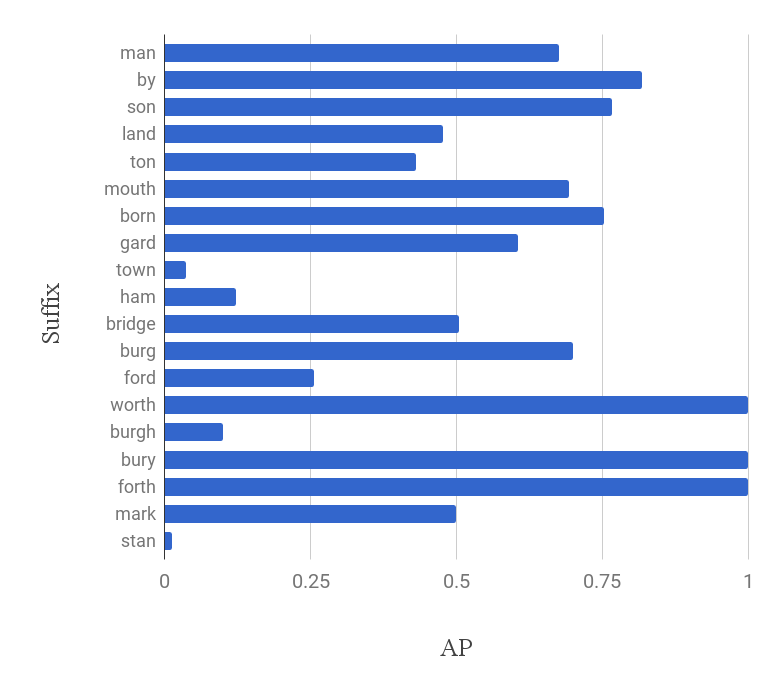
\includegraphics[width=.99\linewidth]{suffix_IAM_ap}
  \caption{A subfigure}
  \label{fig:sub1}
\end{subfigure}%
\begin{subfigure}{.5\textwidth}
  \centering
  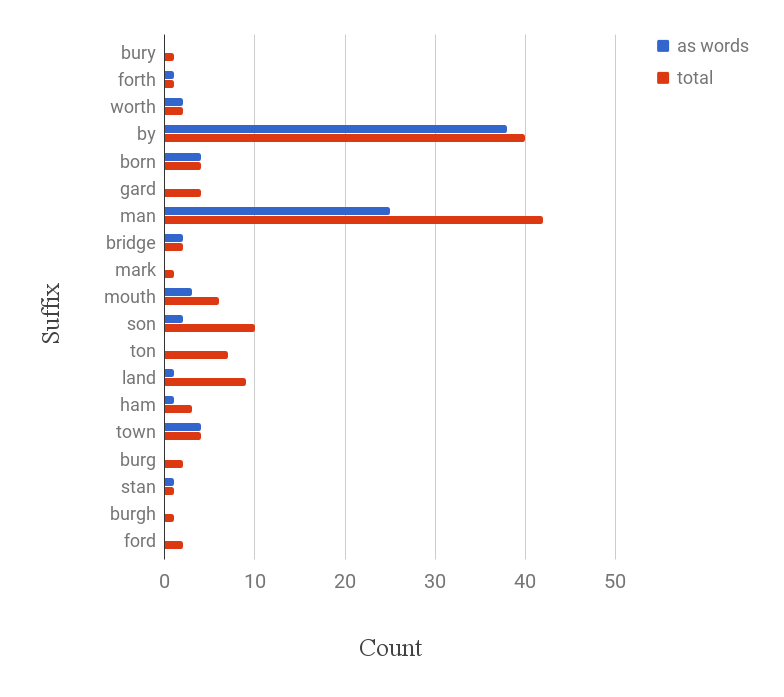
\includegraphics[width=.99\linewidth]{suffix_IAM_count}
  \caption{A subfigure}
  \label{fig:sub2}
\end{subfigure}
\caption{A figure with two subfigures}
\label{fig:test}
\end{figure}


\section{Transcription}

Subword spotting can also be used to transcribe words. There are several ways one could do this, but one of the key aspects that makes subword spotting for transcription appealing is that while subword spotting naturally yields partial transcriptions, matching against a lexicon can constrain the possible full transcriptions resulting from a partial one. We aim towards CAT to better leverage the possibility of user feedback on processes leading to the full transcription.

We describe 4 transcription methods in this section and the results in the following section.
For all methods we used a lexicon. Our primary lexicon consists of 108,028 words and 6,939 names, as described in Chapter \ref{datasets}.

\subsection{Baseline: CAT Through PHOC Vectors}

We use a nearest-neighbors approach as a baseline to transcription using our spotting network, similar to what \cite{krishnan2016} do for word recognition. The PHOC vectors generated by the network on word image are compared to the PHOC vectors of the  words in our lexicon using the Bray-Curtis dissimilarity and the top N matches from the lexicon are returned. This does not use subword spotting, and thus provides a baseline for transcription using our PHOCNet based architecture.







\subsection{CAT Through Approved Subword Spottings}

%overview, and image
\begin{figure}
    \centering
    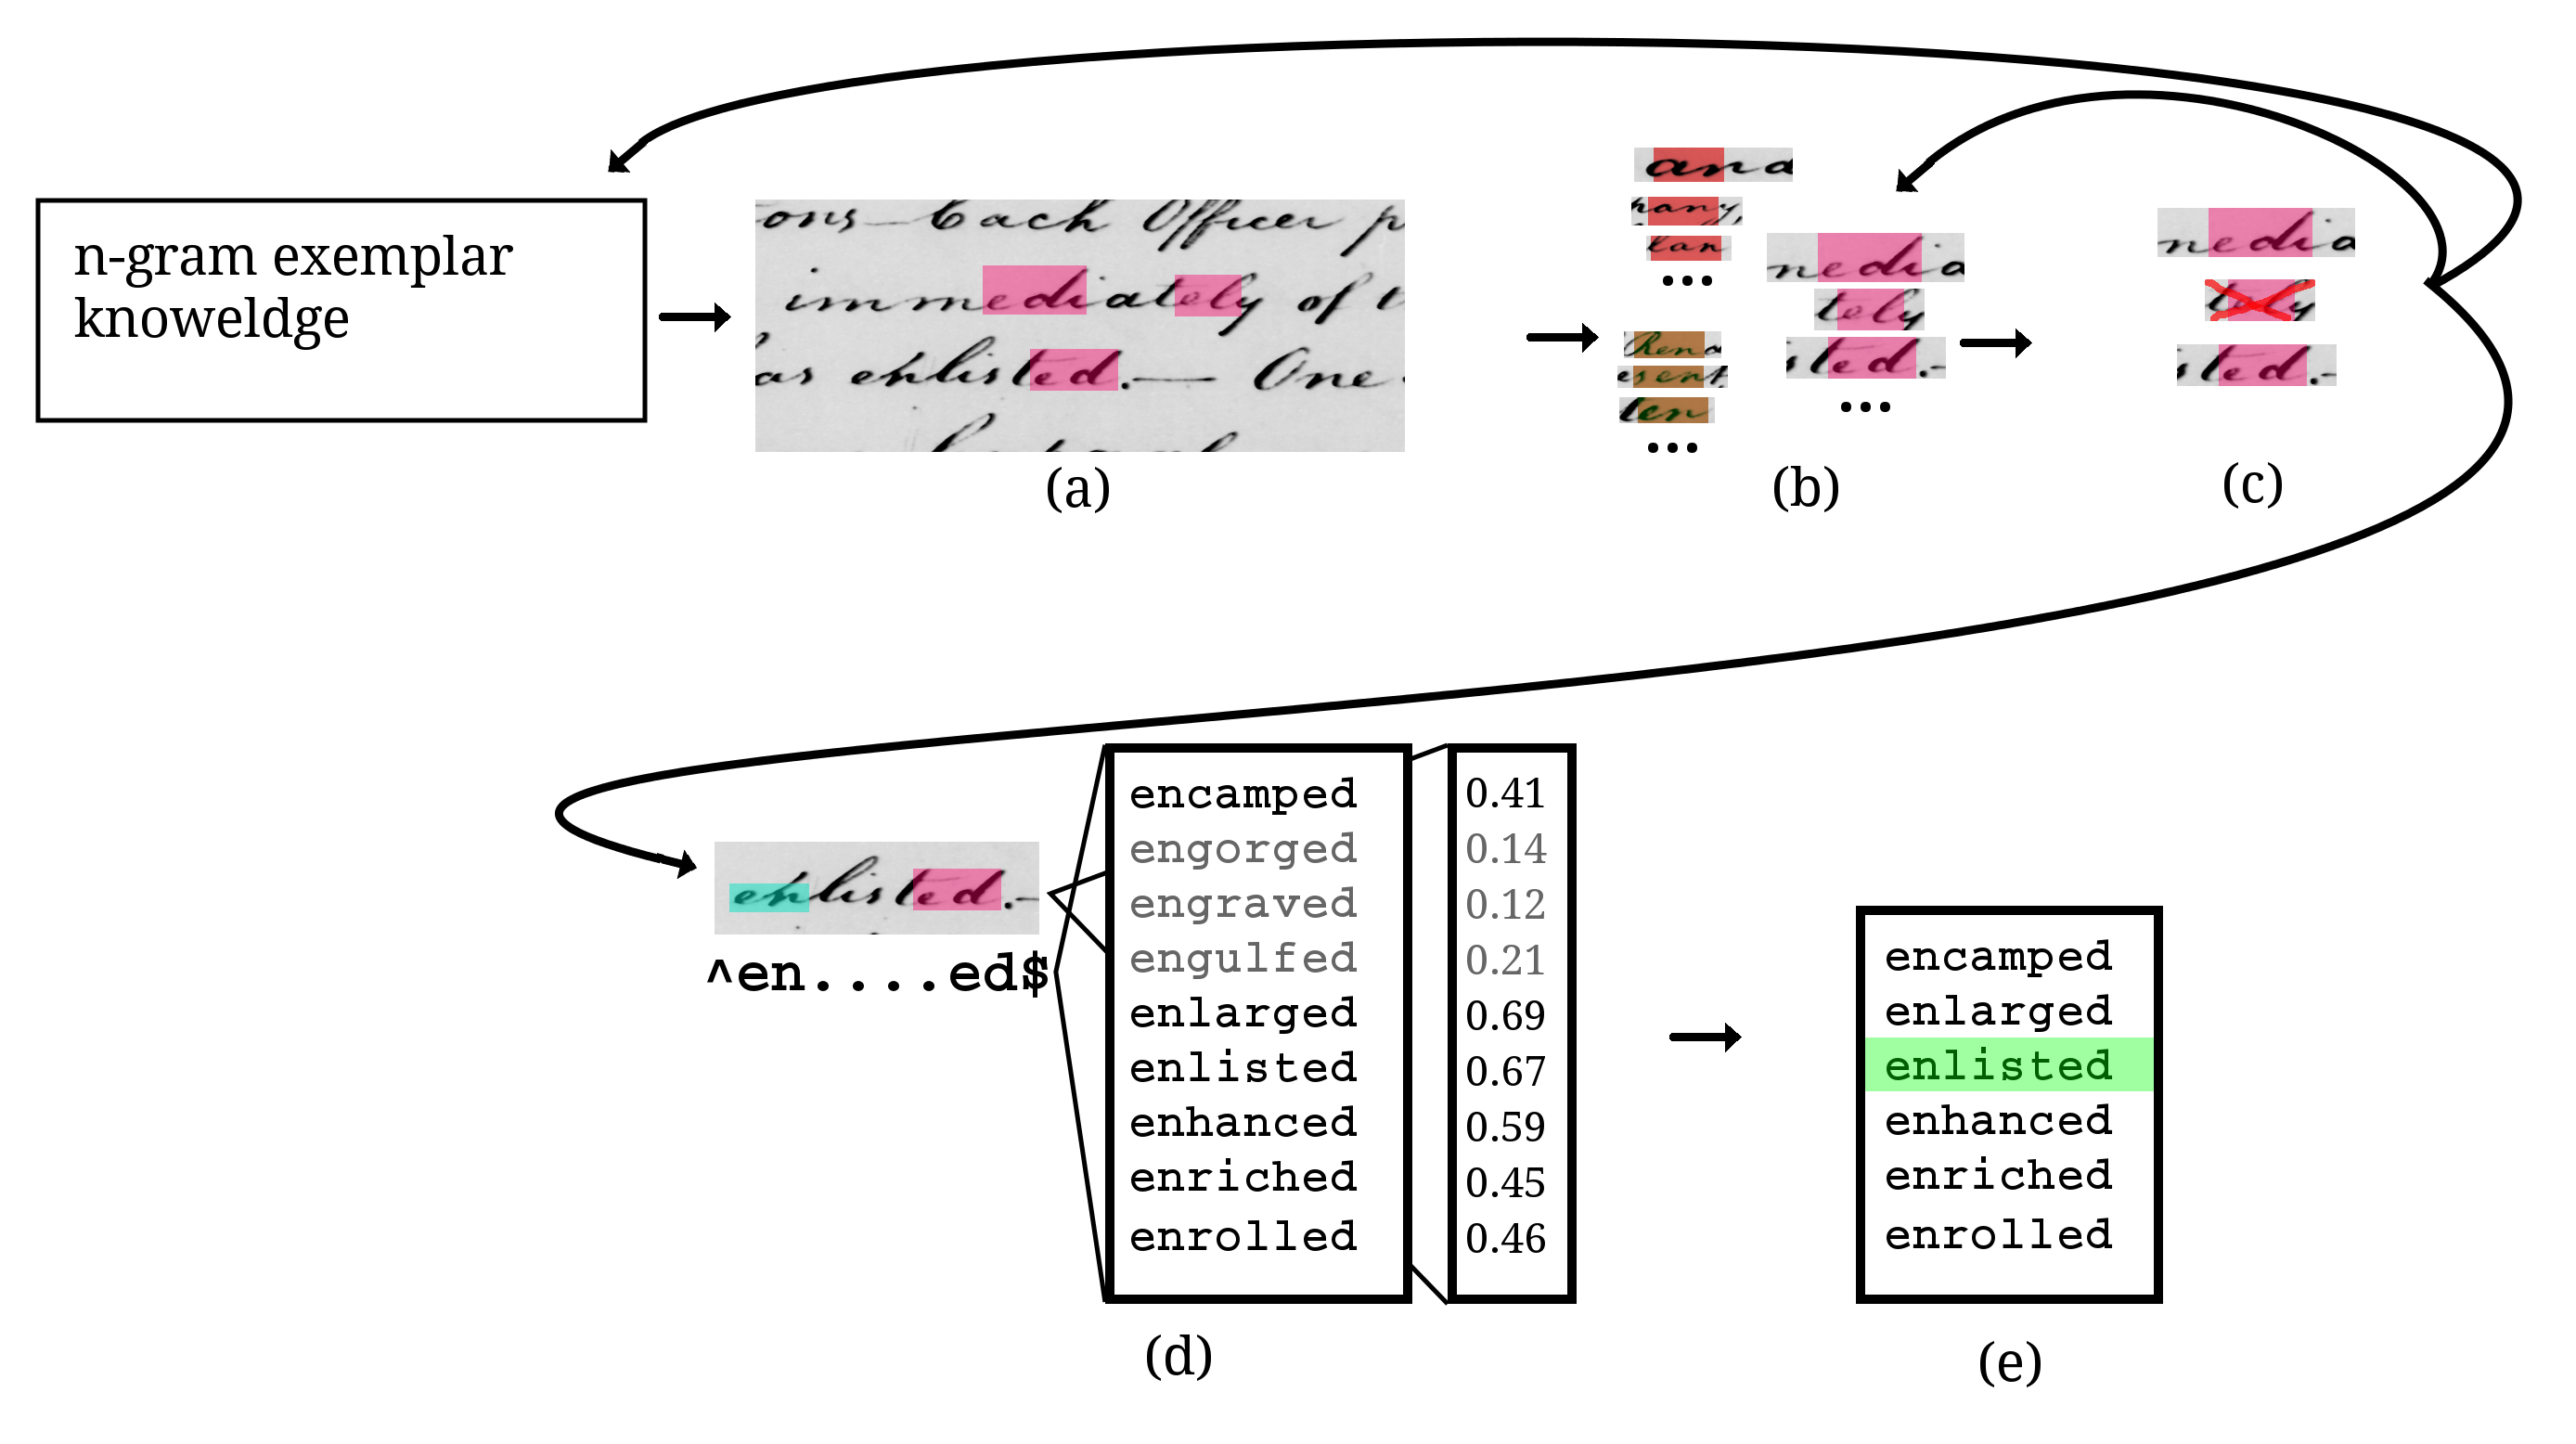
\includegraphics[width=.9\textwidth]{flow6}
    \caption{An overview of the CAT system which uses approved subword spottings. The arrows represent the flow of data.}
    \label{fig:flow}
\end{figure}
An overview of the CAT system using approved subword spotting can be seen in Figure \ref{fig:flow}. Initially the system spots character n-grams in the corpus (word images). These results are pooled and sent to users in batches. After the user identifies correct/incorrect spottings, the spottings' text/label and positions in the word images are used to create regular expressions which is used to query a lexicon for a list of all words matching the constraints set by the spottings. These are scored through word spotting (spotting each lexically relevent word in the image) and lower scores are removed from the list (according to an Otsu threshold). This list is then sent to a user, who selects the correct transcription. Information from approved spottings and transcribed word images can be used in further spottings.

We now go over the individual pieces in greater detail.

\subsubsection{Subword Spotting}
We follow the same procedure for subword spotting as outlined in the Chapter \ref{subwordspotting}. We begin by spotting the n-grams in frequency order, beginning with the largest n using QbS. QbE comes into play after spottings are approved as correct by users. We combine QbE results the same way as described in Section \ref{combine}.
To reduce the number of possible n-grams needing approval, we only return the top portion of all subwindows for a spotting: 75\% for unigrams, 25\% for bigrams, and 15\% for trigrams. The differening percentages reflect the general frequencies of the n-grams in English.

\subsubsection{User Tasks and Interface}

The tasks were intended to be able to be completed on smartphones, but the UI was created as a webapp to increase flexibility to more devices. The webapp requests new batches from the server (system), provides a way for the user to complete the tasks, and sends the completed tasks back to the server.

There are three tasks which need completed: spotting approval, transcription selection, and manual transcription. Spotting approval is rejecting or accepting subword spotting results presented as a word image with a highlighted region. Transcription selection is selecting a correct transcription for a given word image, or correcting spottings displayed on the image. Manual transcription is typing in the transcription for a given word image.

\paragraph{Spotting Approval}

%Should I actually go into the use study? It didn't go through the IRB...
The task which would be presented to users most frequently is spotting approval, as most words will require multiple character n-grams and some spottings will be incorrect. Thus we considered the most effective way to present these to users to reduce the time spent per task.

%Clustering, refer to previous discussion of this? Of discuss here? \cite{Retsinas2015} inspired

Through some trials, we found presenting the potentail n-gram spottings as a list, grouped by the n-gram label, and having the user classify each instance to be efficient. The grouping of spottings with the same n-gram label minimizes context switching and forcing the user to make a decision about each spotting maintains accuracy.

Figure \ref{fig:spottingapproval} shows the interface. The spottings at the bottom is classified as correct or incorrect either with a swipe gesture or a button press. The spottings shown above the current spotting (bottom) allow the user to look ahead and make decisions about the upcoming spottings. The colors of the hilights change when the n-gram label changes to alert the user to the change.

%%%%%%%%%%%%%%
\iffalse
Two modes were developed and tested: a swipe interface and a tap interface. We

\subparagraph{Tap}
In this mode, a batch of 5 spottings were shown together (Figure \ref{im:?}). The user tapped on any incorrect spottings, and then tapped a submit button, after which another batch would be shown. This means that a user can potentially use one action to complete 5 spottings, though it may take 6 actions in the worse case.

\subparagraph{Swipe}
In this mode, the spottings neededing approval queued in a stack with the desired character n-gram being shown at above the stack. see Figure \ref{im:?}. Users either swiped left or right to either reject or accept the spotting shown on the top of the stack. Unlike the tap mode, this forces users to make a decision about each n-gram, potentially increasing accuracy.


\subparagraph{Evaluating Spotting Approval Modes}

fdsgfdh
\fi
%%%%%%%%%%%%%

\paragraph{Transcription Selection}
This task's interface can be seen in Figure \ref{fig:transcriptionselection}.
The user is presented with the image of the word with the spotted n-grams hilighted. Below are the n-gram labels each with an `x' button so the user can indicate an incorrect spotting.
Below these is the list of possible transcriptions. They are presented in an order according to their word spotting score, as this frequently places the correct transcription at the top.
At the end of this list an additional ``Error'' button allows the user to indicate that the correct transcription is not present, and the spotting n-grams are correct.

\paragraph{Manual Transcription}
This task's interface can be seen in Figure \ref{fig:manualtranscription}.
Some words will not be able to be reduced to a short list of possible transcriptions due to poor spotting or possibly errors. These transcriptions must be manually entered by the user. It seems useful to use any known spottings on the given word to provide an intelligent lexicon from which an auto-complete might be able to speed up transcription. However, we observed that generally the spottings were too poor for this assistance to be of much help.



\subsubsection{Word Completion / Regular Expression Generation}\label{wordcompletion}
We rely on the word image width, estimate character width, and the locations of confirmed spottings (spottings approved by user or threshold) in the word to estimate how many characters are likely not spotted in a word. This allows a regular expression to be generated which represents all possible transcriptions of that word.

Spottings are estimated to be a width calculated using the process described in Section \ref{detirminewindowsize}, but without the clustering.
We average these as an approximation of the character width of an unknown character.

The general approach is to measure the number of pixels between each confirmed spotting and divide this by the estimated character width, providing an estimated number of characters (with fractional characters). The range of characters used is 0.8 subtracted and added to this estimate, rounded. The first and last characters are similarly computed, using the beggining and end of the image boundaries as the previous and next spottings, but we additionaly allow each of those ranges to have one less character than computed to account for the fact that frequently first and last letters are longer than others (e.g.~capital letters at the beginning of a word, or a long tail on the last character of a word). If spottings overlap by less than 0.15 the estimated character width, we allow a character to possibly be between them. If spottings overlap and share boundary characters (e.g.~`al' and `le' sharing `l') we permit either a double letter (`alle') or single (`ale') as the spotting methods we use would have trouble distinguishing these situations. Pseudo code is shown in Algorithm \ref{regex}.

%%%%Should be in appendix ?
\begin{algorithm}\label{regex}
 \KwData{Word image width: $W$, List of spottings in word image: $S$ (where $S_i^L$ and $S_i^R$ are the leftmost and rightmost boundary of the $i$th spotting for a word and $S_i^T$ is the n-gram of the spotting), Estimate character width: $C$}
 \KwResult{regular expression for possible transcriptions}
 $i$:=$0$\;
 $p$:=$0$\;
 $r$:=`` ''; (return string)\\
 \While{$i < \text{length of }S$}{
 
  $\delta$:=$S_i^L - p$\;
  $\epsilon$:=$\delta / C$; (estimated number of characters as a float)\\
  
  \eIf{$\epsilon > 0$}{
   $l$:=$\text{floor}(\epsilon)$\;
   $m$:=$\text{ceiling}(\epsilon)$\;
   \If{$\epsilon - l < 0.3$ and $l>0$}{
     $l$:=$l-1$\;
   }
   \If{$m - \epsilon < 0.3$}{
     $m$:=$m+1$\;
   }
   $r$=$r$..``[a-zA-Z0-9]\{$l$,$m$\}''\;
   }{
   (Handling possible overlaps)\\
   $o$:=$\text{length of }S_i^T$\;
   \While{$o>0$}{
     ....\;
     $o$:=$o+1$\;
   }
  }
 }
 \caption{Regular expression generation from spottings.}
\end{algorithm}



Once we have the regular expression, we find all matches in our lexicon.

If there are no matches there are three possible scenarios: the word is not in the lexicon, there is an incorrectly approved spotting, or the spottings and unlabeled characters alignment didn't transfer to the regular expression properly.
To account for the second scenario, we iteratively try removing individual spottings, regenerating the regular expression, and requerying the lexicon to see if matches are found. We make the assumption that only one spotting will be incorrect and union the matching lexicon results. We first only remove spottings that have no overlap (overlap meaning two or more spottings idetified a mutual character) and then those that do.
To account for the third scenario, regenerate the regular expression in a ``loose'' mode, where each range of unknown characters is expanded by one to allow matches initailly constrained by a bad aligment estimation.
If there are no matches and we are already using the ``loose'' regular expression we simply skip the word. It will be manually transcribed eventually.

If there are matches, and the count of them falls below the threshold 49 we score each possible transcription against the image using word spotting.
%That is, we word spot the possible transcription and the word spotting score is used.
As the possible transcriptions are based only on the regular expression, some will be obviously wrong from a visual point of view (e.g.~missing descenders). Following this intuition, we perform an Otsu threshold on the scores to attempt to discard the obviously wrong possibilties. This thresholding is only applied if there are more than 5 possibilities, or if the threshold falls less than half distance between the highest and lowest score (we're confident we're discarding something poor).
If the resulting number of possible transcriptions is less than 7, we package them into a transcription selection task and enqueue it for a user to complete.


\subsubsection{Receiving Transcription}
The user either returns a transcription selection task in three ways: with a selected transcription, with a spotting marked for removal, or with a error indication. These are handeled in the following ways.

If a transcription was selected, that is stored as the transcription for the word. We attempted to extract new ngram image exemplars by interpolating where unspotted n-grams were in the word image, but these generally failed to be good exemplars.

If a spotting is marked for removal, it is removed and the process described in Section \ref{wordcompletion} is followed again, potentailly leading to a new task being enqueued.

If the user indicates an error we first attempt to loosen the regular expression, as described in Section \ref{wordcompletion}. If no matching words are found, we remove the ``worst'' spotting. ``Worst'' first being any spotting labeled by a threshold (not user oversight), and then simply follows the spotting scores.

\subsubsection{Batch Distribution}
ordered list
attempt to find thresholds to accept/reject

checks if all batches in before sending last 12

top, draw best score
guass, draw scores from guassian dist (closest spottings)
fancy-single, draw uniform dist between thresholds
fancy

\subsubsection{Receiving Spotting Approvals}

%\subsubsection{Exemplar extraction}

\subsubsection{Alternate Mode: Don't Wait to Transcribe}
After word spotting lexicon look up (Section \ref{wordcompletion}), return top 7
sdtore others
lexicon lookup

when error on trans, just enqueue next batch

%%%%%%%%%

\subsection{CAT Through Approved Subword Spottings Using Clustering}
sdfgfag


\subsection{CAT Through Unassisted Subword Spotting Using Dynamic Time-Warping Alignment} %

We want to avoid having to make decisions about spottings, either thresholding or having user input, which the previous methods rely on. A way to avoid this is to simply merge all spottings together into a single character probability vector, resulting in something like Figure \ref{fig:cpv}.

\begin{figure}
    \centering
    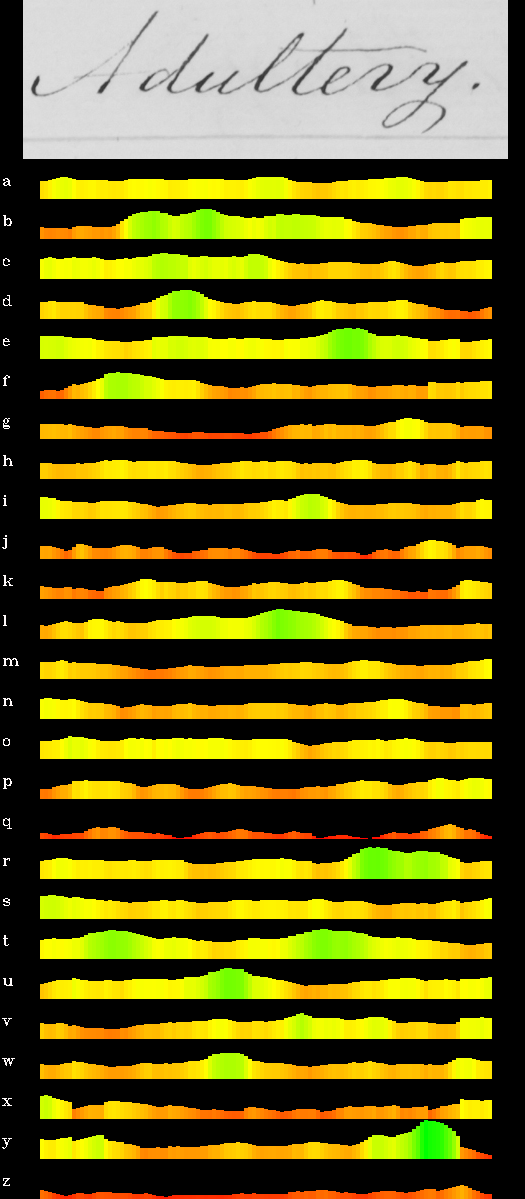
\includegraphics[width=0.5\textwidth]{cpv}
    \caption{An example of a character probability vector for the word ``adultery''. The relative probability of each character (a-z) at each horizontal position is represented both by the height and color of the graph. The discontinuities occuring at the begining and end of the word (e.g. see `x') occur due to the merging of unigram, bigram, and trigram scores.}
    \label{fig:cpv}
\end{figure}

The combining happens according to the following procedure.


\section{Evaluation of Transcription Strategies}
fkjdskglj

top 5 acc for CTC: 0.584546 OLD


%%%%%%%%%%%%%%%%%%%%%%%%%%%%%%%%%%%%%%%%%%%%%%%%%%%%%%%%%%%%%%%%%%%%%%%%%%%%%%


%%%%%%%%%%%%%%%%%%%%%%%%%%%%%%%%%%%%%%%%%%%%%%%%%%%%%%%%%%%%%%%%%%%%%%%%%%%%%%
%\chapter{System Testing and Results}

%blah blah

%%%%%%%%%%%%%%%%%%%%%%%%%%%%%%%%%%%%%%%%%%%%%%%%%%%%%%%%%%%%%%%%%%%%%%%%%%%%%%
\chapter{Conclusion}

\section{Contributions}

1. Subword spotting evaluation
2. Applications of subword spotting
3. Transcription (RegEx, combining 1,2,3)
4. Crowd source

\section{Future Work}

deslant
segmentation free

regex search/spotting
CPV to regex

%\nocite{testentry}

\bibliographystyle{plainnat}
\bibliography{bib}

\end{document}

% vim: lbr
